\documentclass[10pt,a4paper]{book}

\NewDocumentCommand\esp{}{\;}
\NewDocumentCommand\noise{}{\varepsilon}
\NewDocumentCommand\Estep{}{\textit{E-step}}
\NewDocumentCommand\Mstep{}{\textit{M-step}}
\NewDocumentCommand\kmean{}{$k$-\textit{means}}

% 今後の方向性
% 強化学習
% 共役勾配法または準ニュートン法による深層学習の実験

% 編集方針
% モデルの説明に変数tを使わず、全てy \simeq f(x)に統一する
% 正解や標本などの難しそうな用語とカタカナ語の使用を控える
% ベクトル変数や教師データの添字や集合の表現の使用を控える
% サンプルコードにある変数やクラス名の具体的な言及を控える

\book{Scalaで実装するパターン認識と機械学習}{Scala's Pattern Recognition {\&} Machine Learning}{3}{機械学習,データマイニング}

\begin{document}
\maketitle
\tableofcontents

\chapter{初歩的な機械学習モデル\label{chap:intro}}

機械学習とは、説明変数$\bm{x}$と目的変数$\bm{y}$の組$\XY$の集合$\TRAIN$から、変数$\bm{x},\bm{y}$の関係を表す関数$f$を推定する方法である。
集合$\TRAIN$が、関数$f$の取る値$\bm{y}$を具体的に列挙する場合は、その問題を\textbf{教師あり学習}と呼び、集合$\TRAIN$を\textbf{教師データ}と呼ぶ。
%
\begin{equation}
\forall\bm{x},\bm{y}\colon \pair{\bm{x}}{\bm{y}}\in\TRAIN \Rightarrow \bm{y} \approx f(\bm{x}).
\end{equation}
%
教師あり学習で、目的変数$\bm{y}$が、\textbf{クラス}と呼ばれる離散値を取る場合を\textbf{分類}と呼ぶ。その初歩的な例が\textbf{最近傍法}である。
最近傍法では、未知の点$\bm{x}$のクラスは、$\bm{x}$の至近距離にある既知の$K$個の点の多数決で決まる。\subfigref{knn}{model}に例を示す。

\begin{figure}[h]
\centering
\subfloat[$k$ nearest neighbor diameters.\label{fig:knn:model}]{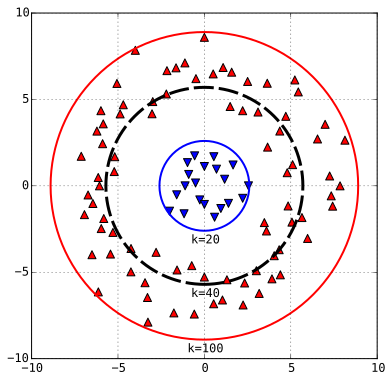
\includegraphics[width=.5\linewidth]{images/knn.model.eps}}
\subfloat[$k\!=\!10$ region segmentation.\label{fig:knn:class}]{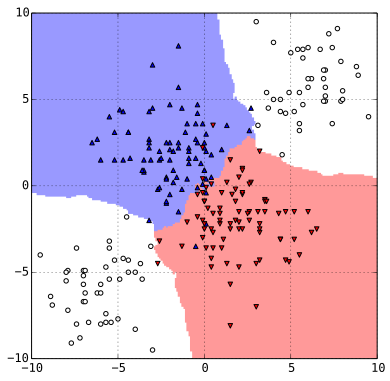
\includegraphics[width=.5\linewidth]{images/knn.class.eps}}
\caption{$k$ nearest neighbor model.\label{fig:knn}}
\end{figure}

\subfigref{knn}{class}は、各々が正規分布に従う3クラスの点の集合を学習し、空間全体をそれらのクラスに分類した結果である。
最近傍法では、適当な距離関数$d$を使う。距離関数$d$は、\eqref{knn:dist}の\textbf{距離の公理}を満たし、任意の2点の距離を定義する。
%
\begin{equation}
\label{eq:knn:dist}
\forall \bm{x},\bm{y},\bm{z} \in \mathbb{R}^D \colon
0 \leq d(\bm{x},\bm{y}) = d(\bm{y},\bm{x}) \leq d(\bm{x},\bm{z}) + d(\bm{z},\bm{y}),\esp
\bm{x} = \bm{y} \Leftrightarrow d(\bm{x},\bm{y}) = 0.
\end{equation}
%
最近傍法は、他の著名な教師あり学習の手法と比較して、事前の学習が不要である点が特徴的で、\textbf{遅延学習}と呼ばれる。
以上の議論に基づき、最近傍法を実装しよう。引数は、参照する近傍点の個数$K$と、集合$\seq{\bm{x},y}$と、距離関数$d$である。

\begin{Verbatim}{Scala}
class KNN[D,T](k: Int, data: Seq[(D,T)], d: (D,D)=>Double) {
	def apply(x: D) = data.sortBy((p,t)=>d(x,p)).take(k).groupBy((p,t)=>t).maxBy((g,s)=>s.size)._1
}
\end{Verbatim}

使用例を以下に示す。距離関数の例として、初等幾何学の基礎であるユークリッド距離や\textbf{マンハッタン距離}を使用した。
後者は、座標の差の絶対値の総和を距離とする。距離関数の最適な選択肢は、分類対象の問題の性質に応じて変化する。

\begin{Verbatim}{Scala}
val samples2d = Seq.fill(100)(Seq.fill(2)(util.Random.nextGaussian) -> util.Random.nextBoolean)
val euclidean = new KNN(5, samples2d, (a,b) => math.sqrt(a.zip(b).map((a,b)=>(a-b)*(a-b)).sum))
val manhattan = new KNN(5, samples2d, (a,b) => a.zip(b).map(_-_).map(_.abs).sum)
\end{Verbatim}

\section{線型回帰}

教師あり学習で、目的変数$\bm{y}$が連続な値を取る場合を\textbf{回帰}と呼ぶ。その代表的な例が、\textbf{線型回帰}である。\eqref{lbf:basis}に示す。
適当な基底関数$\phi$の線型結合である。基底関数は、関数$f$の形に応じて選ぶ。例えば、多項式基底やガウス基底を使う。
%
\begin{equation}
\label{eq:lbf:basis}
\bm{y} + \noise \approx f(\bm{x}) = \sum_{k=0}^K w_k \phi_k(\bm{x}) = \trans{\bm{w}}\bm{\phi}(\bm{x}).
\end{equation}
%
基本的に、変数$\bm{x},\bm{y}$は誤差$\noise$を含む。例えば、映像や音声信号には、\eqref{lbf:noise}に示す、分散$\sigma^2$の\textbf{ガウスノイズ}が重畳する。
%
\begin{equation}
\label{eq:lbf:noise}
y \sim
\Lk{f} =
\prob{y}[\bm{x},f] =
\Nd{y}{f(\bm{x}),\sigma^2} =
\frac{1}{\sqrt{2\pi}\sigma}\exp\left\{-\frac{(y-f(\bm{x}))^2}{2\sigma^2}\right\}.
\end{equation}
%
\eqref{lbf:noise}の確率は、確率$f$の妥当性と見做せる。これを\textbf{尤度}と呼ぶ。尤度の最大値を探せば、最適な関数$\hat{f}$が推定できる。
これを\textbf{最尤推定}と呼び、機械学習の基本原理である。尤度の対数から、\eqref{lbf:error}が導出される。関数$E$を2乗誤差と呼ぶ。
%
\begin{equation}
\label{eq:lbf:error}
\hat{f} =
\argmax_f \log \prob{y}[\bm{x},f] =
\argmin_f \seq{y-f(\bm{x})}^2 =
\argmin_f E(\bm{w}).
\end{equation}
%
誤差$E$を削減する方向に加重$\bm{w}$を動かす操作を繰り返すと、極小点に収束する。これを\textbf{勾配法}と呼ぶ。\eqref{lbf:grad}に示す。
%
\begin{equation}
\label{eq:lbf:grad}
\hat{\bm{w}} = \bm{w} - \eta \nabla E(\bm{w}) = \bm{w} + \eta \sum_{n=1}^N \{y_n - \trans{\bm{w}} \bm{\phi}(\bm{x}_n)\} \bm{\phi}(\bm{x}_n),
\where
\eta \ll \abs{\frac{\bm{w}}{\nabla E(\bm{w})}}.
\end{equation}
%
定数$\eta$を\textbf{学習率}と呼ぶ。以上の議論に基づき、線型回帰を実装する。引数は、学習率$\eta$と、集合$\seqxy$と、基底$\Phi$である。

\begin{Verbatim}{Scala}
class Regression(e: Double, data: Seq[(Double,Double)], p: Seq[Double=>Double], epochs: Int = 1000) {
	val w = Array.fill[Double](p.size)(0)
	def apply(x: Double) = w.zip(p.map(_(x))).map(_ * _).sum
	for(n <- 1 to epochs; (x,y) <- data) w.zip(p).map(_ + e * (y - this(x)) * _(x)).copyToArray(w)
}
\end{Verbatim}

\figref{lbf}は、多項式基底とガウス基底を利用して、各々の基底に適した形状の曲線に対し、線型回帰を行った結果である。

\begin{figure}[h]
\centering
\subfloat[$\seq{x^3,x^2,x,1}$]{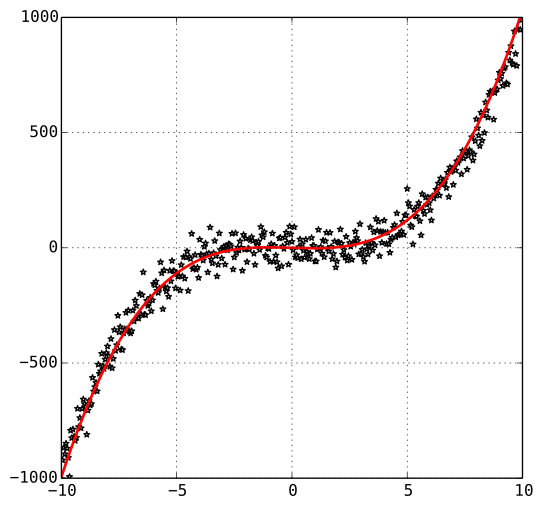
\includegraphics[width=.5\linewidth]{images/lbf.power.eps}}
\subfloat[$G(x|\pm5, 1)$]{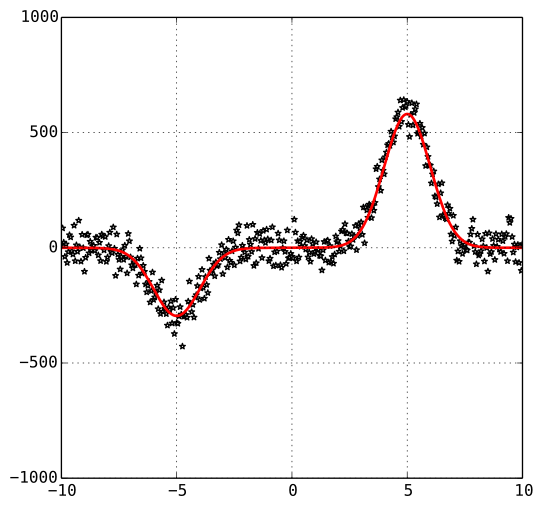
\includegraphics[width=.5\linewidth]{images/lbf.gauss.eps}}
\caption{linear basis function model.\label{fig:lbf}}
\end{figure}

なお、加重$\bm{w}$は最適化されたが、基底関数$\Phi$自体は最適化されず、\textbf{ハイパーパラメータ}として扱った点に注意を要する。

\section{単純ベイズ分類器}

自然言語で記述された記事の話題を分類する問題を考える。記事$d$は単語$w_n$の列であり、単語は話題$c$から生成される。
記事$d$の内容を話題$c$と仮定する。この仮説の尤度は、単語の共起を無視すれば、\eqref{nbc:pdc}の条件付き確率で定義される。
%
\begin{equation}
\label{eq:nbc:pdc}
\Lk{c} =
\Prob{d}[c] =
\Prob{w_1,\dots,w_{N_d}}[c] =
\prod_{n=1}^{N_d} \Prob{w_n}[c,w_1,...,w_{n-1}] \simeq
\prod_{n=1}^{N_d} \Prob{w_n}[c].
\end{equation}
%
最適な話題$\hat{c}$は、\eqref{nbc:pcd}の条件付き確率を最大化する。確率$\Prob{c}$は記事$d$とは独立した確率で、\textbf{事前確率}と呼ばれる。
\eqref{nbc:pcd}は、記事$d$を観測した後の話題$c$の確率で、これを\textbf{事後確率}と呼ぶ。\eqref{nbc:pcd}の変形は、\textbf{ベイズの定理}を使った。
%
\begin{equation}
\label{eq:nbc:pcd}
\hat{c} =
\argmax_c \Prob{c}[d] =
\argmax_c \frac{\Prob{c}\Prob{d}[c]}{\Prob{d}} =
\argmax_c \Prob{c}\Prob{d}[c] =
\argmax_c \Prob{c} \prod_{n=1}^{N_d} \Prob{w_n}[c].
\end{equation}
%
ただし、初めて出現した単語$w$に対して、\eqref{nbc:pcd}の確率が$0$になる事態を防ぐため、\eqref{nbc:smooth}の\textbf{ラプラス平滑化}を行う。
%
\begin{equation}
\label{eq:nbc:smooth}
\Prob{w}[c] =
\frac{\Prob{w,c}}{\Prob{c}} \simeq
\frac{N_{wc}+1}{N_c+1} > 0,
\Leftarrow
\Prob{w} = \frac{1}{\abs{V}},
\where
N_c = \sum_{w \in V} N_{wc}.
\end{equation}
%
変数$N_{wc}$は、組$\pair{w}{c}$の頻度である。\eqref{nbc:smooth}は、単語$w$の事前確率を\chapref{lda}で学ぶディリクレ分布と仮定して導かれる。
\eqref{nbc:pcd}の分類器を\textbf{単純ベイズ分類器}と呼ぶ。以下に実装を示す。引数は、既知の記事の列と、対応する話題の列である。

\begin{Verbatim}{Scala}
class NaiveBayes[D<:Seq[W],W,C](texts: Seq[D], classes: Seq[C]) {
	val nw = scala.collection.mutable.Map[(W,C),Double]().withDefaultValue(1)
	val pc = classes.groupBy(identity).map(_ -> _.size.toDouble / texts.size)
	def pwc(c: C)(w: W) = nw(w,c) / texts.flatten.distinct.map(nw(_,c)).sum
	def pcd(d: D)(c: C) = math.log(pc(c)) + d.map(pwc(c)).map(math.log).sum
	def apply(d: D) = classes.distinct.maxBy(pcd(d))
	for((d,c) <- texts.zip(classes); w <- d) nw(w,c) += 1
}
\end{Verbatim}

\subfigref{nbc:jmap}{8}は、百科事典で各地方の記事から固有名詞を抽出して学習し、都道府県の記事の地方を推定した結果である。

\begin{figure}[h]
\centering
\subfloat[8-regional division.\label{fig:nbc:jmap:8}]{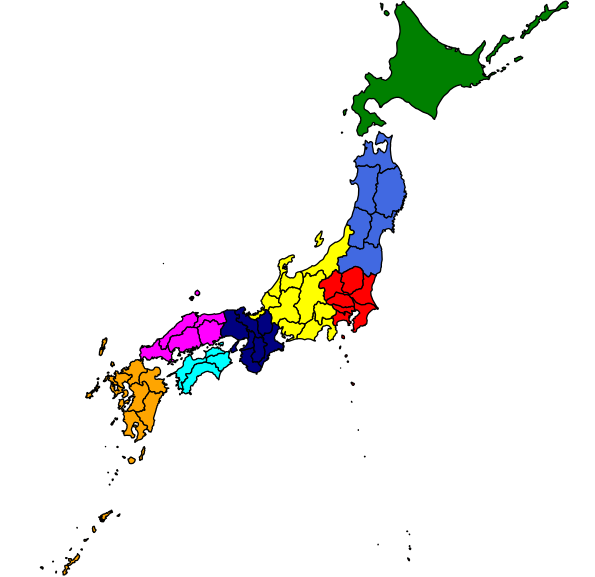
\includegraphics[width=.5\linewidth]{images/nbc.jmap8.eps}}
\subfloat[2-regional division.\label{fig:nbc:jmap:2}]{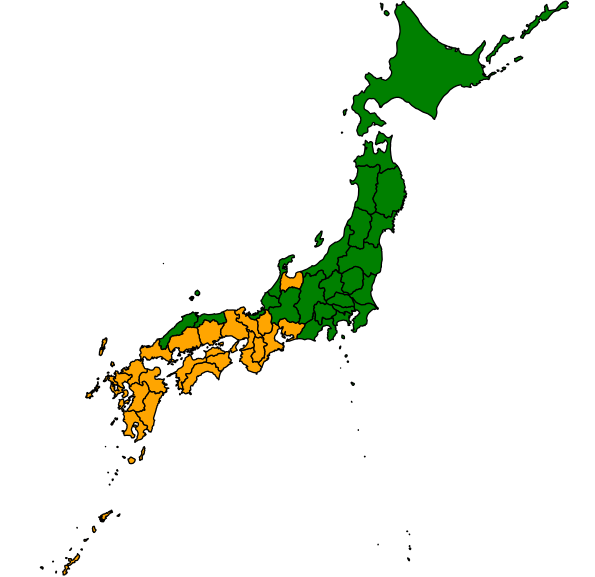
\includegraphics[width=.5\linewidth]{images/nbc.jmap2.eps}}
\caption{Japanese map division into regions based on classification of Wikipedia pages.\label{fig:nbc:jmap}}
\end{figure}

\subfigref{nbc:jmap}{2}は、東日本と西日本の記事を学習して、都道府県を分類した結果である。単純だが、高精度な分類ができる。

\chapter{ニューラルネットワーク\label{chap:nn}}

\textbf{ニューラルネットワーク}は、線型回帰に似た\textbf{ニューロン}と呼ばれる関数を連結して、連鎖構造にした複雑な関数である。
単体のニューロンは、線型回帰の後に、\textbf{活性化関数}と呼ばれる非線型な関数$f$を適用した関数で、\eqref{nn:neuron}で定義される。
%
\begin{equation}
\label{eq:nn:neuron}
\bm{y} \simeq f(\bm{z}) = f(W\bm{x}).
\end{equation}
%
単体では、線型回帰と同じ程度の表現能力だが、何層も重ねることで、任意の\textbf{滑らかな関数}を任意の精度で近似できる。
循環構造がなく、直線的な構造の\textbf{順伝播型}の動作は、\eqref{mlp:fp}の漸化式で定義できる。循環構造の場合は\sectref{rnn}で扱う。
%
\begin{equation}
\label{eq:mlp:fp}
\bm{y}_n = \bm{x}_{n+1} = f_n(\bm{z}_n) = f_n(W_n\bm{x}_n).
\end{equation}
%
\eqref{mlp:fp}で、第$n$層は前の層から値$\bm{x}_n$を受容し、行列$W_n$で加重して活性化関数$f_n$を適用し、後続の層に値$\bm{y}_n$を渡す。
活性化関数には、\textbf{シグモイド関数}が広く利用される。\eqref{nn:sigm}に定義する。これは、2クラスの分類器のように振る舞う。
%
\begin{equation}
\label{eq:nn:sigm}
\sigm(z) = \frac{1}{1 + e^{-z}} = \frac{1}{2}\tanh\frac{z}{2} + \frac{1}{2}.
\end{equation}
%
代表的な活性化関数の例を\subfigref{slp}{trans}に示す。他には、\eqref{slp:smax}に示す\textbf{ソフトマックス関数}も特に最終層で利用される。
%
\begin{equation}
\label{eq:slp:smax}
y \sim \hatprob{y} = \smax(\bm{z}) =
\frac{1}{e^{z_1}+\cdots+e^{z_K}}
\begin{pmatrix}
e^{z_1}\\
\vdots\\
e^{z_K}
\end{pmatrix}.
\end{equation}
%
最終層の活性化関数を適切に選ぶと、回帰や分類など、様々な問題に対応できる。特に分類問題の例は\sectref{smax}に述べる。
\subfigref{slp}{class}は、活性化関数にシグモイド関数を利用し、論理和を求める例である。直線$f(\bm{x})=0.5$は分類の境界を表す。

\begin{figure}[h]
\centering
\subfloat[activation functions.\label{fig:slp:trans}]{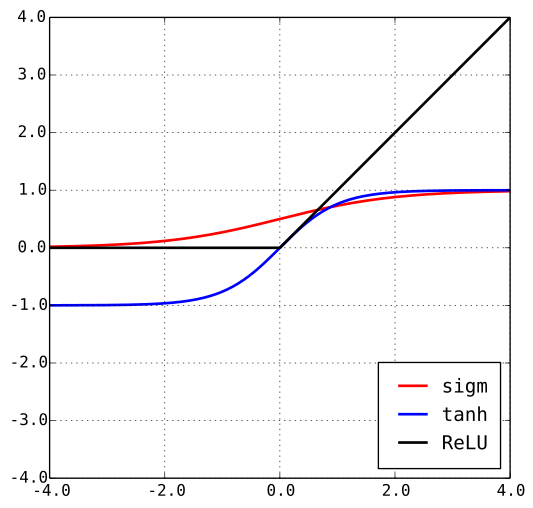
\includegraphics[width=.5\linewidth]{images/slp.trans.eps}}
\subfloat[OR learned by neuron.\label{fig:slp:class}]{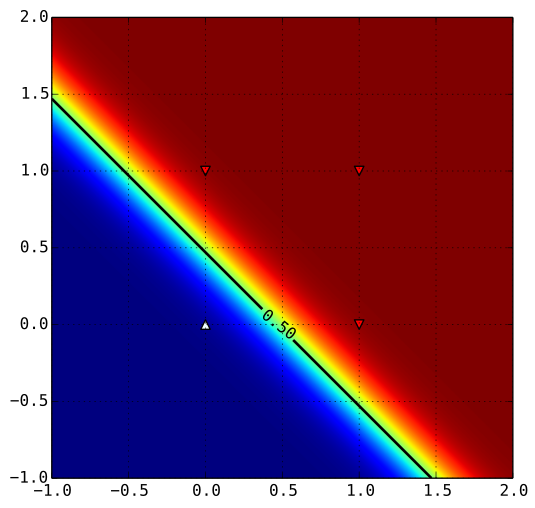
\includegraphics[width=.5\linewidth]{images/slp.class.eps}}
\caption{neuron mechanism.\label{fig:slp}}
\end{figure}

論理和や論理積は、分類の境界が直線や超平面となる単純な問題で、これを\textbf{線型分離可能}と呼び、単層でも表現できる。
\chapref{nn}で学ぶ誤差逆伝搬法は、多数の層を訓練して、線型分離が困難な問題に適合させる\textbf{深層学習}を支える技法である。

\section{誤差逆伝播法の理論\label{sect:mlp}}

深層学習では、多数の層の加重を最適化して、誤差$E$を最小化する。最適解の計算は困難なので、逐次的に最適化する。
具体的な手順は、以下の通りである。まず、第$n$層の加重$W_n$を最適化の対象とし、\eqref{mlp:sgd}に示す勾配法で最適化する。
%
\begin{equation}
\label{eq:mlp:sgd}
w_n'^{ij}
= w_n^{ij}-\eta \pdiff{E}{w_n^{ij}}
= w_n^{ij}-\eta \pdiff{z_n^j}{w_n^{ij}} \pdiff{x_{n+1}^j}{z_n^j} \pdiff{E}{x_{n+1}^j}
= w_n^{ij}-\eta x_n^i \pdiff{f}{z_n^j}(z_n^j) \pdiff{E}{x_{n+1}^j}.
\end{equation}
%
定数$\eta$は学習率で、変数$x_n^i,z_n^j$は、変数$\bm{x}_n,\bm{z}_n$の第$i,j$成分である。さて、\eqref{mlp:fp}から\eqref{mlp:bp}の漸化式が導出される。
\eqref{mlp:bp}の漸化式を利用して、誤差$E$を逆方向に伝播させ、\eqref{mlp:sgd}の最適化を各層で行う。これを\textbf{誤差逆伝播法}と呼ぶ。
%
\begin{equation}
\label{eq:mlp:bp}
\pdiff{E}{x_n^i}
= \sum_{j=1}^J \pdiff{z_n^j}{x_n^i} \pdiff{x_{n+1}^j}{z_n^j} \pdiff{E}{x_{n+1}^j}
= \sum_{j=1}^J w_n^{ij} \pdiff{f}{z_n^j}(z_n^j) \pdiff{E}{x_{n+1}^j}.
\end{equation}
%
漸化式の初期値を考える。2乗誤差関数$\Esq$を仮定すると、最終層の値$\hat{\bm{y}}$と目的変数$\bm{y}$に対し、導関数は\eqref{mlp:gE:sq}になる。
%
\begin{equation}
\label{eq:mlp:gE:sq}
\pdiff{\Esq}{\hat{y}^j} = \pdiff{}{\hat{y}^j} \frac{1}{2} \norm{\bm{y}-\hat{\bm{y}}}^2,
\where
\Esq(\hat{\bm{y}},\bm{y}) = \frac{1}{2} \norm{\bm{y}-\hat{\bm{y}}}^2.
\end{equation}
%
\eqref{mlp:bp}には、活性化関数の微分が含まれるが、活性化関数は巧妙に設計されており、実に単純な四則演算で計算できる。
%
\begin{equation}
\label{eq:nn:sigm:d}
\pdiff{\sigm}{z_n^j}(z_n^j) = \frac{e^{-z_n^j}}{(1+e^{-z_n^j})^2} = x_{n+1}^j(1-x_{n+1}^j).
\end{equation}
%
\sectref{chain}では、誤差逆伝播法を備えると同時に、自在に層構造を定義可能な深層学習を実装する。利用方法を以下に示す。

\begin{Verbatim}{Scala}
val model3 = new Output(1, _-_)
val model2 = new Offset(3, new Sigmoid, ()=>new PlainSGD, model3)
val model1 = new Offset(2, new Sigmoid, ()=>new PlainSGD, model2)
for(n <- 1 to 1000000; x <- 0 to 1; y <- 0 to 1) model1.bp(Seq(x,y), Seq(x^y))
\end{Verbatim}

複数の非線型変換を持つ恩恵で、線型分離が困難な分類問題にも対応できる。具体例として、排他的論理和を学習する。
通常の結果を\subfigref{mlp.split}{class}に、各層の変数$\bm{x}$に定数項を含む場合の結果を\subref{fig:mlp.split:const}に示す。定数項の有無で、境界が変化した。

\begin{figure}[h]
\centering
\subfloat[\texttt{Hidden + Hidden}.\label{fig:mlp.split:class}]{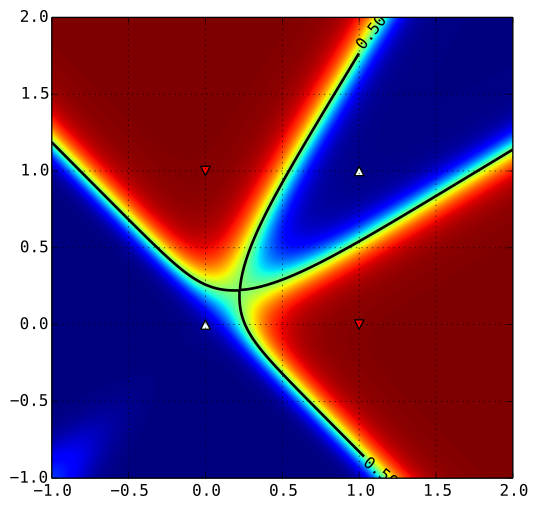
\includegraphics[width=.5\linewidth]{images/mlp.class.eps}}
\subfloat[\texttt{Offset + Offset}.\label{fig:mlp.split:const}]{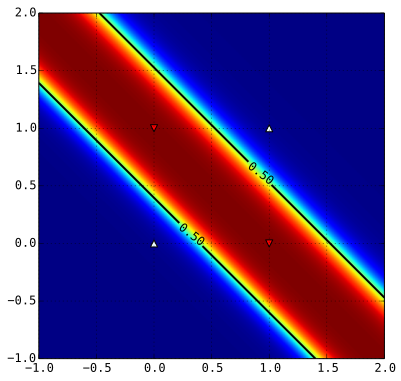
\includegraphics[width=.5\linewidth]{images/mlp.const.eps}}
\caption{exclusive OR learned by a three-layer perceptron.\label{fig:mlp.split}}
\end{figure}

ぜひ実装して、学習の途中経過を観察しよう。また、加重の初期値によって、収束までの時間が変わる様子も観察できる。

\section{誤差逆伝播法の実装\label{sect:chain}}

以上の数式を実装し、誤差$E$を逆伝播させ、最終層から最初層まで逐次的に最適化しよう。最初に、勾配法を定義する。

\begin{Verbatim}{Scala}
abstract class SGD(var w: Double = math.random) extends (Double => Unit)
\end{Verbatim}

これは、加重$w$の抽象化であり、\eqref{mlp:sgd}による最適化も行う。具体的な最適化の手順は、勾配法を継承して実装する。

\begin{Verbatim}{Scala}
class PlainSGD(e: Double = 0.01) extends SGD {
	def apply(dE: Double): Unit = this.w -= e * dE
}
\end{Verbatim}

引数は、学習率$\eta$である。学習時は、誤差$E$の勾配$\nabla E$を受け取り、加重$w$を修正する。次に、活性化関数を定義する。

\begin{Verbatim}{Scala}
trait Act {
	def fp(z: Seq[Double]): Seq[Double]
	def bp(y: Seq[Double]): Seq[Double]
}
\end{Verbatim}

活性化関数は、順伝播と逆伝播を行う。以下に、具体的な実装例を示す。順伝播は\eqref{nn:sigm}に、逆伝播は\eqref{nn:sigm:d}に従う。

\begin{Verbatim}{Scala}
class Sigmoid extends Act {
	def fp(z: Seq[Double]) = z.map(z => 1 / (1 + math.exp(-z)))
	def bp(z: Seq[Double]) = this.fp(z).map(y => y * (1.0 - y))
}
\end{Verbatim}

次に、層を定義する。加重と活性化関数を持ち、順伝播と逆伝播を行う中間層と、誤差関数を計算する最終層が派生する。

\begin{Verbatim}{Scala}
abstract class Neuron(val dim: Int) {
	def fp(x: Seq[Double]): Seq[Double]
	def bp(x: Seq[Double], t: Seq[Double]): Seq[Double]
}
\end{Verbatim}

最終層を実装する。引数は、最終層が出力する値の要素数と、誤差の導関数である。誤差関数は、\textbf{損失関数}とも呼ばれる。

\begin{Verbatim}{Scala}
class Output(dim: Int = 1, loss: (Double,Double)=>Double = _-_) extends Neuron(dim) {
	def fp(x: Seq[Double]) = x
	def bp(x: Seq[Double], t: Seq[Double]) = x.zip(t).map(loss.tupled)
}
\end{Verbatim}

中間層も実装する。引数は、中間層が受け取る値の要素数と、活性化関数と、加重を生成する関数と、後続の層である。

\begin{Verbatim}{Scala}
class Hidden(dim: Int, act: Act, weight: ()=>SGD, next: Neuron) extends Neuron(dim) {
	lazy val w = List.fill(next.dim, dim)(weight())
	def fp(x: Seq[Double]) = next.fp(act.fp(wx(x)))
	def wx(x: Seq[Double]) = w.map(_.map(_.w).zip(x).map(_ * _).sum)
	def bp(x: Seq[Double], t: Seq[Double]) = ((z: Seq[Double]) => {
		val bp = next.bp(act.fp(z),t).zip(act.bp(z)).map(_ * _)
		for((w,g) <- w.zip(bp); (sgd,x) <- w.zip(x)) sgd(x * g)
		w.transpose.map(_.zip(bp).map(_.w * _).sum)
	})(wx(x))
}
\end{Verbatim}

最後に、定数項を実装する特殊な中間層も実装する。仕組みは単純で、中間層が受け取る値に定数$1$の要素を追加する。

\begin{Verbatim}{Scala}
class Offset(dim: Int, act: Act, weight: ()=>SGD, next: Neuron) extends Neuron(dim) {
	lazy val body = new Hidden(dim + 1, act, weight, next)
	def fp(x: Seq[Double]) = body.fp(x.padTo(dim + 1, 1d))
	def bp(x: Seq[Double], t: Seq[Double]) = body.bp(x.padTo(dim + 1, 1d), t).init
}
\end{Verbatim}

\section{ソフトマックス関数\label{sect:smax}}

\textbf{多クラス分類}の問題では、最終層の活性化関数に\eqref{slp:smax}のソフトマックス関数とし、各クラスの確率分布$p$を学習する。
誤差関数には、\eqref{smax:ce}の\textbf{交差エントロピー}を使う。\eqref{smax:ce}の$H(p)$は、確率分布$p$の不偏性を表す\textbf{平均情報量}である。
%
\begin{equation}
\label{eq:smax:ce}
\Ece(p,\hatp) =
-\int \prob{\bm{y}} \log \hatprob{\bm{y}} d\bm{y} =
-\int \prob{\bm{y}} \left\{\log \prob{\bm{y}} - \log\frac{\prob{\bm{y}}}{\hatprob{\bm{y}}}\right\} d\bm{y} =
H(p) + \KL{p}{\hatp} \geq
\KL{p}{\hatp}.
\end{equation}
%
\eqref{smax:KL}の$\KL{p}{\hatp}$を\textbf{カルバック・ライブラー情報量}と呼ぶ。これは非負で、確率分布$p,\hatp$が等価な場合に限り$0$になる。
\eqref{smax:KL}から確率分布$\hatp$の項を抽出すると、分布$\hatp$の対数の期待値である。また、分布$\hatp$は各層の加重$W_n$の尤度である。
%
\begin{equation}
\label{eq:smax:KL}
\KL{p}{\hatp} =
\int_K \prob{y} \log \frac{\prob{y}}{\hatprob{y}} dy \geq \int_K \prob{y} \tup{1-\frac{\hatprob{y}}{\prob{y}}} dy = 0.
\end{equation}
%
分類器が推定する確率分布$\hatp$を真の確率分布$p$に近付けるには、\eqref{smax:ce}を最小化し、間接的に\eqref{smax:KL}を最小化する。
これは、尤度$\hatp$の対数の期待値の最大化に相当し、即ち最尤推定である。例えば、最終層では\eqref{smax:gE}の勾配法を行う。
%
\begin{equation}
\label{eq:smax:gE}
\pdiff{\Ece}{z^k}
= - \pdiff{}{z^k} \sum_{i=1}^K y^i \tup{\log e^{z^i} - \log \sum_{j=1}^K e^{z^j}}
= - y^k + \sum_{i=1}^K y^i \hat{y}^k = -y^k + \hat{y}^k.
\end{equation}
%
以上の議論を踏まえ、\eqref{slp:smax}の順伝播と\eqref{smax:gE}の勾配計算を実装する。この活性化関数は、最終層でのみ使用できる。

\begin{Verbatim}{Scala}
class Softmax extends Act {
	def fp(z: Seq[Double]) = z.map(math.exp(_)/z.map(math.exp).sum)
	def bp(z: Seq[Double]) = Seq.fill(z.size)(1.0)
}
\end{Verbatim}

勾配$\nabla f(\bm{z})$の計算を誤魔化したので、中間層で使うと、逆伝播が妨害される。その点に目を瞑れば、簡単に実装できた。

\begin{Verbatim}{Scala}
val model = new Offset(3, new Softmax, ()=>new PlainSGD, new Output(4, _-_))
\end{Verbatim}

\figref{mcp.zflag}は、国際信号旗の\textit{Z}旗を学習する例である。問題が簡単なので、単層の方が多層よりも正確な\textit{Z}旗を学習できる。

\begin{figure}[h]
\centering
\subfloat[2-layer perceptron]{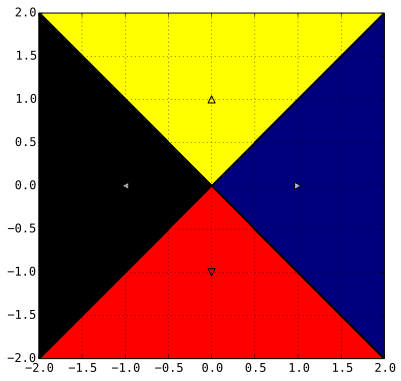
\includegraphics[width=.5\linewidth]{images/slp.zflag.eps}}
\subfloat[3-layer perceptron]{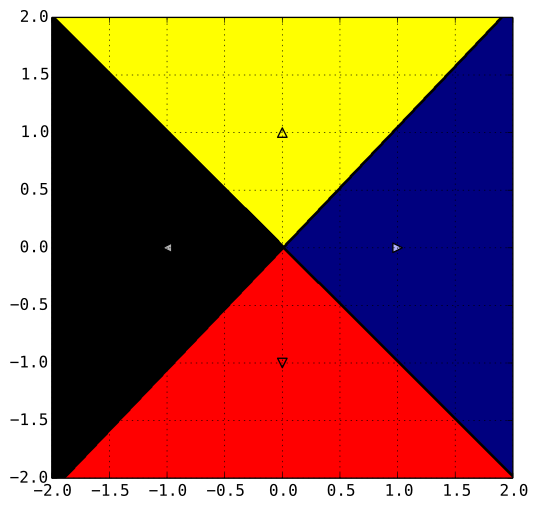
\includegraphics[width=.5\linewidth]{images/mlp.zflag.eps}}
\caption{maritime signal flag \textit{zulu} learned by a perceptron.\label{fig:mcp.zflag}}
\end{figure}

層を増やすと、表現能力は高まるが、\sectref{nn.sgd}でも述べる通り、学習が停滞しやすく、却って精度が低下する場合がある。

\section{鞍点と学習率の調整\label{sect:nn.sgd}}

勾配法には、最適解に到達する前に\textbf{鞍点}で最適化が停滞する場合がある。\eqref{sgd:saddle}に示す関数$E$の最小化の例で考える。
鞍点とは、ある方向では極大値だが、別の方向では極小値となる停留点である。関数$E$の場合は、原点$\bm{O}$が鞍点である。
%
\begin{equation}
\label{eq:sgd:saddle}
\Delta E = \pdiff{f}{x} \Delta x + \pdiff{f}{y} \Delta y = 2x \Delta x - 2y \Delta y,
\where
E(x,y) = x^2 - y^2.
\end{equation}
%
原点$\bm{O}$に嵌ると、\subfigref{sgd}{avoid}のように最適化が止まる。しかし、$y\neq0$に動けば、勾配が負になり、最適化を再開できる。
鞍点は頻繁に現れる。\subfigref{sgd}{speed}は、5通りの初期値で排他的論理和を学習した際の誤差$\Esq$の推移で、停滞が見られる。

\begin{figure}[h]
\centering
\subfloat[saddle point avoidance mechanism.\label{fig:sgd:avoid}]{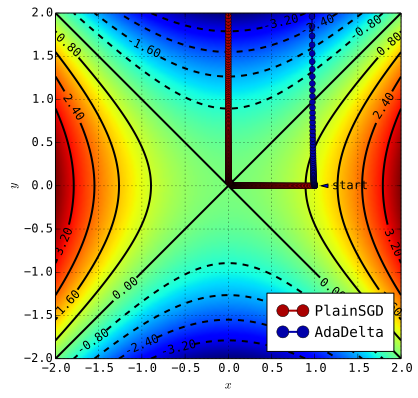
\includegraphics[width=.5\linewidth]{images/sgd.avoid.eps}}
\subfloat[loss diminution through training.\label{fig:sgd:speed}]{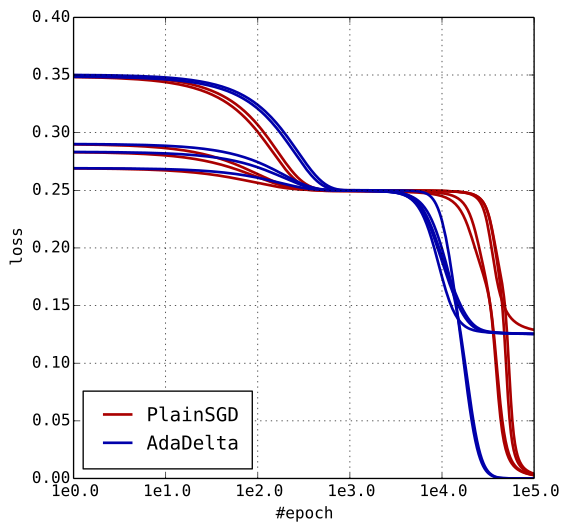
\includegraphics[width=.5\linewidth]{images/sgd.speed.eps}}
\caption{comparison of \texttt{PlainSGD} and \texttt{AdaDelta}.\label{fig:sgd}}
\end{figure}

対策として、最適解の近傍では学習率を小さく、鞍点の近傍で学習率を大きく調節する、適応的な勾配法が利用される。
例えば、\eqref{sgd:adagrad}の\textit{AdaGrad}は、時刻$t$での学習率を勾配$\nabla E_t$の期待値の逆数とし、また、時刻$t$に従って減衰させる。
%
\begin{equation}
\label{eq:sgd:adagrad}
\Delta w = -\frac{\eta}{t\sqrt{\E{(\nabla E)^2}_t}},
\where
\left\{
\begin{aligned}
\E{(\nabla E)^2}_t &= \frac{1}{t} \sum_{\tau=0}^t (\nabla E_\tau)^2, \\
\E{(\nabla E)^2}_0 &= \varepsilon.
\end{aligned}
\right.
\end{equation}
%
\textit{AdaGrad}は全時間の勾配を考慮するが、\eqref{sgd:adadelta}の\textit{AdaDelta}では、期待値に加重$\rho$を導入し、直近の勾配を重視する。
\eqref{sgd:adadelta}の分数には、加重$w$と勾配$\nabla E$の単位を変換する役割がある。なお、定数$\varepsilon$はゼロ除算を防ぐ微小な値である。
%
\begin{equation}
\label{eq:sgd:adadelta}
\Delta w_{mt} = -\frac{\sqrt{\E{(\Delta w)^2}_t+\varepsilon}}{\sqrt{\E{(\nabla E)^2}_t+\varepsilon}} \nabla E_{mt},
\where
\left\{
\begin{aligned}
\E{x}_t &= \rho \E{x}_{t-1} + (1-\rho) x_t, \\
\E{x}_0 &= 0.
\end{aligned}
\right.
\end{equation}
%
以上の議論を踏まえ、\textit{AdaDelta}を実装する。引数は、定数$\rho,\varepsilon$である。\figref{sgd}に、単純な勾配法との性能の比較を示す。

\begin{Verbatim}{Scala}
class AdaDelta(r: Double = 0.95, e: Double = 1e-8) extends SGD {
	var eW, eE = 0.0
	def apply(dE: Double) = {
		lazy val v = math.sqrt(eW + e) / math.sqrt(eE + e)
		this.eE = r * eE + (1 - r) * math.pow(1 * dE, 2.0)
		this.eW = r * eW + (1 - r) * math.pow(v * dE, 2.0)
		this.w -= v * dE
	}
}
\end{Verbatim}

\section{通時的誤差逆伝播法\label{sect:rnn}}

自然言語や信号など、時系列の未来を予測するには、状態を記憶し、時系列を逐次的に順伝播させる機能が必要である。
\textbf{再帰型ニューラルネットワーク}が代表的で、中間層の状態$\bm{y}$を、次の時刻の入力$\bm{x}$の順伝播に合流させ、中間層に戻す。
%
\begin{equation}
\label{eq:nn:rnn}
\bm{y}^t = f(\bm{z}^t) = f(W_i\bm{x}^t+W_h\bm{y}^{t-1}).
\end{equation}
%
再帰構造を展開して、擬似的に再帰を除去すれば、従来通り勾配法で最適化できる。これを\textbf{通時的誤差逆伝播法}と呼ぶ。
以下に実装を示す。順伝播は、同じ中間層を繰り返し通過し、最後に、後続の層に伝播する。逆伝播も、同様に実装する。

\begin{Verbatim}{Scala}
class RNN(dim: Int, hidden: Neuron, output: Neuron, value: Double = 0) extends Neuron(dim) {
	val hist = Seq[Seq[Double]]().toBuffer
	val loop = Seq[Seq[Double]]().toBuffer
	def fp(x: Seq[Double]) = output.fp(hp(x).last)
	def tt(x: Seq[Double]) = hist.zip(loop).map(_++_).foldRight(x)
	def hp(x: Seq[Double]) = loop.append(hidden.fp(hist.append(x).last++loop.last))
	def bp(x: Seq[Double], t: Seq[Double]) = tt(output.bp(hp(x).last,t))(hidden.bp)
	def init = hist.clear -> loop.clear -> loop.append(Seq.fill(hidden.dim)(value))
}
\end{Verbatim}

順伝播や逆伝播を行う度に、中間層の状態が記憶される。従って、時系列の処理が終わる度に、初期化する必要がある。
勾配法も実装し直す。逆伝播の間に、中間層の挙動が変わると最適化に障るので、逆伝播の完了まで、加重を据え置く。

\begin{Verbatim}{Scala}
class DelaySGD(sgd: SGD = new PlainSGD, var d: Double = 0) extends SGD {
	def apply(dE: Double) = (sgd.w = w, sgd(dE), d += sgd.w - w)
	def force = (w += d, d = 0)
}
\end{Verbatim}

使用例を示す。なお、中間層で逆伝播を繰り返す際に、勾配は引数で渡される。その勾配を、専用の最終層で取り出す。

\begin{Verbatim}{Scala}
val params = Seq[DelaySGD]().toBuffer
val model3 = new Offset(5, new Sigmoid, ()=>params.append(new DelaySGD).last, new Output(1))
val model2 = new Offset(6, new Sigmoid, ()=>params.append(new DelaySGD).last, new Output(5, (x,e)=>e))
val model1 = new RNN(1, model2, model3)
\end{Verbatim}

時系列の具体的な例として、波形を学習させる。余弦波を受け取り、位相を遅らせて正弦波を予測する回帰問題である。

\begin{Verbatim}{Scala}
val x = Seq.tabulate(200)(n => Seq(0.5 * math.cos(0.02 * math.Pi * n) + 0.5))
val y = Seq.tabulate(200)(n => Seq(0.5 * math.sin(0.02 * math.Pi * n) + 0.5))
for(step <- 1 to 100000) model1.init -> x.zip(y).foreach(model1.bp(_,_) -> params.foreach(_.force))
\end{Verbatim}

\figref{rnn}に予測した波形と真の波形を示す。学習の初期段階では、歪な波形だが、学習が進むと、綺麗な正弦波に近付く。

\begin{figure}[h]
\centering
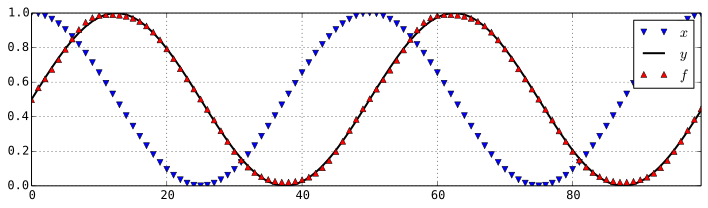
\includegraphics[width=\linewidth]{images/rnn.phase.eps}
\caption{sine curve prediction.\label{fig:rnn}}
\end{figure}

時系列の機械学習は、機械翻訳や映像生成など、発展が顕著な分野で、複雑な文脈構造を如何に捉えるかが課題である。

\chapter{サポートベクターマシン}

\textbf{サポートベクターマシン}は、分類問題に対し、各クラスの集団からの距離$d$が最大になる境界を学習する分類器である。
\subfigref{svm}{l}に線型分離可能な問題の、\figsubref{svm}{c}に線型分離が困難な問題の例を示す。まずは、線型分離可能な場合を解説する。

\begin{figure}[h]
\centering
\subfloat[linear problem.\label{fig:svm:l}]{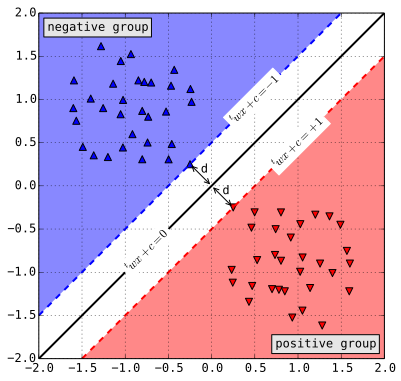
\includegraphics[width=.5\linewidth]{images/svm.model.eps}}
\subfloat[curved problem.\label{fig:svm:c}]{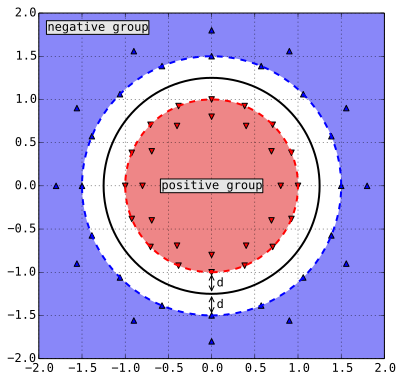
\includegraphics[width=.5\linewidth]{images/svm.round.eps}}
\caption{a support vector machine.\label{fig:svm}}
\end{figure}

\subfigref{svm}{l}の分類器は、\eqref{svm:class}に従って、説明変数$\bm{x}$に対し、目的変数$y$を推定する。$\bm{w}$は加重で、$c$は定数項である。
%
\begin{equation}
\label{eq:svm:class}
\hat{y} = \sign{\dprod{\bm{w}}{\bm{x}}+c} \in \seq{1,-1}.
\end{equation}
%
距離$d$の最適化は\textbf{制約付き最適化問題}であり、学習対象の集合$\TRAIN$に対して、\eqref{svm:hard}に示す制約条件を満たす必要がある。
%
\begin{equation}
\label{eq:svm:hard}
\forall \pair{\bm{x}}{y} \in \TRAIN \colon y(\dprod{\bm{w}}{\bm{x}} + c) \geq 1,
\where
y\in\seq{1,-1}.
\end{equation}
%
距離$d$は\eqref{svm:d}で求まる。\eqref{svm:hard}を念頭に、式を簡略化すると、距離$d$の最大化は加重$\bm{w}$の最小化と等価だと言える。
%
\begin{equation}
\label{eq:svm:d}
d(\TRAIN) = \min\frac{\abs{\dprod{\bm{w}}{\bm{x}} + c}}{\norm{\bm{w}}} = \frac{1}{\norm{\bm{w}}},
\where
\bm{x}\in\TRAIN.
\end{equation}
%
現実には、\eqref{svm:hard}の\textbf{ハードマージン}は、誤分類に対して過剰に敏感なので、\eqref{svm:soft}に示す\textbf{ソフトマージン}を利用する。
%
\begin{equation}
\label{eq:svm:soft}
\forall \pair{\bm{x}}{y} \in \TRAIN \colon
y (\dprod{\bm{w}}{\bm{x}} + c) \geq 1 - \xi,
\where
\xi =
\begin{cases}
0 & \text{if $y(\dprod{\bm{w}}{\bm{x}} + c) > 1$}, \\
\abs{y - (\dprod{\bm{w}}{\bm{x}} + c)} \geq 0 & \text{if $y(\dprod{\bm{w}}{\bm{x}} + c) \leq 1$}.
\end{cases}
\end{equation}
%
\eqref{svm:soft}は、誤分類された点$\bm{x}$に対し、罰を与える役割がある。$\xi$を\textbf{ヒンジ損失}と呼ぶ。最終的に\eqref{svm:main}を最小化する。
%
\begin{equation}
\label{eq:svm:main}
f(\bm{w}) = C \sum_n^N \xi_n + \frac{1}{2}\norm{\bm{w}}^2,
\where
C>0.
\end{equation}
%
定数$C$は、誤分類の許容量を決定する。小さな値に設定すると誤分類に鈍感になり、大きな値に設定すると敏感になる。

\section{双対問題の導出}

\eqref{svm:main}は、\eqref{svm:soft}を束縛条件として、\textbf{ラグランジュの未定乗数法}で最小化できる。条件が2個ある点に注意を要する。
%
\begin{equation}
\label{eq:svm:L}
L(\bm{w},c,\xi,\lambda,\mu,\TRAIN) =
f(\bm{w}) - \sum_{i=1}^N \lambda_n \{y_n(\dprod{\bm{w}}{\bm{x}_n} + c) - 1 + \xi_n\} - \sum_{i=1}^N \mu_n \xi_n.
\end{equation}
%
\eqref{svm:soft}の条件は不等式なので、\eqref{svm:kkt}の\textbf{カルーシュ・クーン・タッカー条件}を満たす場合のみ、未定乗数法が使える。
%
\begin{equation}
\label{eq:svm:kkt}
\lambda_n \seq{y_n\tup{\dprod{\bm{w}}{\bm{x}_n} + c} - 1 + \xi_n} = 0,\esp
\left\{
\begin{aligned}
\lambda_n &\geq 0, \\
\mu_n     &\geq 0, \\
\mu_n\xi_n&=0.
\end{aligned}
\right.
\end{equation}
%
変数$\lambda_n,\mu_n$は未定乗数である。\eqref{svm:L}を加重$\bm{w}$と定数$c$と未定乗数で偏微分すれば、$L$が極値になる条件が得られる。
%
\begin{equation}
\label{eq:svm:best}
\pdiff{L}{w} = \pdiff{L}{c} = \pdiff{L}{\lambda} = \pdiff{L}{\mu} = 0,
\Rightarrow
\left\{
\begin{aligned}
\bm{w}    &= \sum_{i=1}^N \lambda_n y_n \bm{x}_n, \\
0         &= \sum_{i=1}^N \lambda_n y_n, \\
\lambda_n &= C - \mu_n.\\
\end{aligned}
\right.
\end{equation}
%
\subfigref{svm}{l}を振り返ると、$C=0$の場合は、\eqref{svm:kkt}より、境界から距離$d$の点だけが$\lambda>0$となり、加重$\bm{w}$に寄与する。
その点を\textbf{サポートベクトル}と呼ぶ。\eqref{svm:L}に\eqref{svm:best}を代入すると、都合よく$\xi$や$C$が消去され、\eqref{svm:dual}が得られる。
%
\begin{equation}
\label{eq:svm:dual}
\tilde{L}(\lambda) =
\min_{\bm{w},c} L(\bm{w},c, \lambda) =
\sum_{i=1}^N \lambda_i \seq{1 - \frac{1}{2} \sum_{j=1}^N \lambda_j y_i y_j (\dprod{\bm{x}_i}{\bm{x}_j})} \leq f(\bm{w}).
\end{equation}
%
\eqref{svm:dual}の$\tilde{L}$の最大化を$f(\bm{w})$の\textbf{ラグランジュ双対問題}と呼ぶ。$\tilde{L}$と$f(\bm{w})$の最適値は合致する。これを\textbf{強双対性}と呼ぶ。

\section{逐次的な最適化\label{sect:smo}}

\eqref{svm:dual}の解析的な最適化は困難なため、\textbf{逐次最小問題最適化法}での最適化を検討する。まず、適当な2点$\bm{x}_i,\bm{x}_j$を選ぶ。
その2点の乗数$\lambda_i,\lambda_j$を\eqref{smo:d}を満たす範囲で最適化する。以上の操作を、全ての点が\eqref{svm:kkt}を満たすまで繰り返す。
%
\begin{equation}
\label{eq:smo:d}
y_i \delta_i + y_j \delta_j = 0,
\where
\left\{
\begin{aligned}
\delta_i &= \hat{\lambda}_i - \lambda_i \\
\delta_j &= \hat{\lambda}_j - \lambda_j
\end{aligned}
\right\}
\Leftarrow 0 = \sum_{i=1}^N \lambda_i y_i.
\end{equation}
%
2点$\bm{x}_i,\bm{x}_j$に対し、$\tilde{L}$の極大値を求める。\eqref{smo:d}に注意して、\eqref{svm:dual}を$\delta_i,\delta_j$で偏微分すると、\eqref{smo:dL}が得られる。
%
\begin{equation}
\label{eq:smo:dL}
\pdiff{\tilde{L}}{\delta_i} = y_i (y_i-y_j)-\delta_i \abs{\bm{x}_i-\bm{x}_j}^2-y_i \sum_{n=1}^N \lambda_n y_n \dprod{\bm{x}_n}{(\bm{x}_i-\bm{x}_j)}.
\end{equation}
%
乗数$\lambda_i,\lambda_j$の移動量は\eqref{smo}となる。ただし、\eqref{svm:kkt}を満たす必要があり、$0\leq\lambda\leq C$の範囲で\textbf{クリッピング}を行う。
%
\begin{equation}
\label{eq:smo}
\delta_i = -\frac{y_i}{\abs{\bm{x}_i-\bm{x}_j}^2} \seq{\sum_{n=1}^N \lambda_n y_n \dprod{\bm{x}_n}{(\bm{x}_i-\bm{x}_j)}-y_i+y_j}.
\end{equation}
%
なお、定数$c$の値は、$y(\dprod{\bm{w}}{\bm{x}})$を最小化する点$\bm{x}$に着目すると、\eqref{smo:c}で計算できる。以上で、必要な数式が出揃った。
%
\begin{equation}
\label{eq:smo:c}
c = -\frac{1}{2} \seq{
\min_{i|y_i=+1} \sum_{j=1}^N \lambda_j y_j \dprod{\bm{x}_i}{\bm{x}_j} +
\max_{j|y_j=-1} \sum_{i=1}^N \lambda_i y_i \dprod{\bm{x}_j}{\bm{x}_j}}.
\end{equation}
%
逐次最小問題最適化法の最悪計算時間は$O(n^3)$だが、点$\bm{x}_i$を選ぶ際に、\eqref{svm:kkt}に反する点を重視すると効率的である。

\section{線型分離の学習}

\sectref{smo}までの議論に基づき、逐次最小問題最適化法を実装する。まず、組$\pair{\bm{x}}{y}$を実装する。乗数$\lambda$を変数として持つ。

\begin{Verbatim}{Scala}
case class Data(x: Seq[Double], t: Int, var l: Double = 0) {
	def kkt(svm: SVM, C: Double) = t * svm(this) match {
		case e if e < 1 => l >= C
		case e if e > 1 => l == 0
		case _ => true
	}
}
\end{Verbatim}

次に、サポートベクターマシンの本体を実装する。引数\texttt{k}は内積である。敢えて抽象化したのは、\sectref{kernel}の布石である。

\begin{Verbatim}{Scala}
class SVM(data: Seq[Data], k: (Data, Data) => Double) {
	var const = 0.0
	def group(t: Int) = data.filter(_.t == t).map(apply)
	def apply(x: Data) = data.map(d => d.l * d.t * k(x,d)).sum + const
}
\end{Verbatim}

最後に、逐次最小問題最適化法を実装する。\sectref{smo}に述べた数式を実装し、\eqref{svm:kkt}を満たすまで逐次的に最適化する。

\begin{Verbatim}{Scala}
class SMO(data: Seq[Data], k: (Data, Data) => Double, C: Double = 1e-10) extends SVM(data,k) {
	while(data.filterNot(_.kkt(this,C)).size >= 2) {
		val a = data(util.Random.nextInt(data.size))
		val b = data(util.Random.nextInt(data.size))
		val min = math.max(-a.l, if(a.t == b.t) b.l - this.C else -b.l)
		val max = math.min(-a.l, if(a.t == b.t) b.l - this.C else -b.l) + C
		val prod = this(Data(a.x.zip(b.x).map(_-_), 0)) - this.const
		val best = -a.t * (prod - a.t + b.t) / (k(a,a) - 2 * k(a,b) + k(b,b))
		if(!best.isNaN) a.l += a.t * a.t * math.max(min, math.min(max, best))
		if(!best.isNaN) b.l -= a.t * b.t * math.max(min, math.min(max, best))
		this.const = -0.5 * (group(+1).min + group(-1).max) + this.const
	}
}
\end{Verbatim}

\figref{svm:line}に学習の例を示す。綺麗な境界を学習できた。\figsubref{svm:line}{2}では、誤分類によりサポートベクトルが消える様子がわかる。

\begin{figure}[h]
\centering
\subfloat[sample data separable by a line.\label{fig:svm:line:1}]{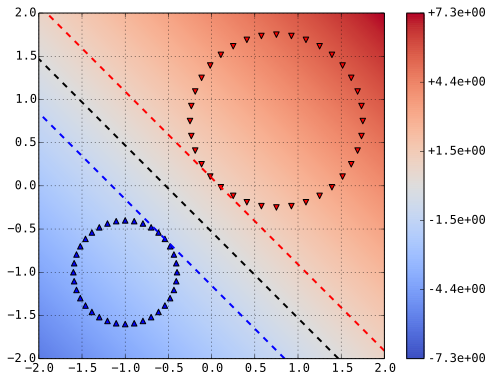
\includegraphics[width=.5\linewidth]{images/svm.line1.eps}}
\subfloat[sample data with outlier points.\label{fig:svm:line:2}]{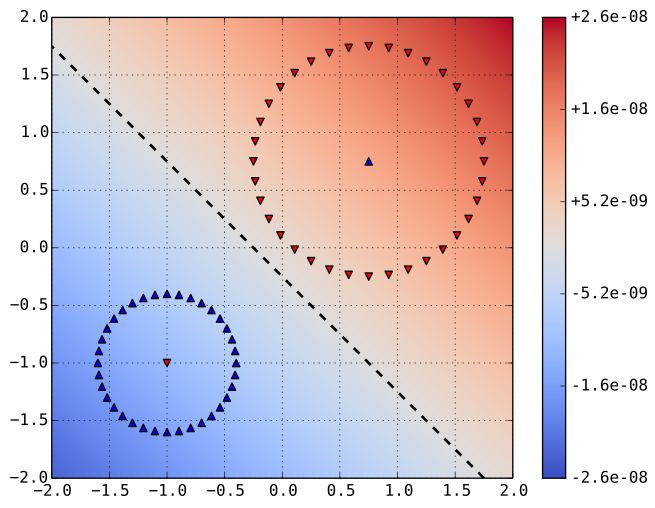
\includegraphics[width=.5\linewidth]{images/svm.line2.eps}}
\caption{decision surface learned by a linear SVM.\label{fig:svm:line}}
\end{figure}

黒の点線はクラスの境界を表し、赤と青の点線はサポートベクトルを表す。赤と青の濃淡は$\dprod{\bm{w}}{\bm{x}}+c$の値の勾配を表す。

\section{特徴空間の変換\label{sect:kernel}}

\sectref{smo}までの議論は、線型分離可能な問題が前提だった。\sectref{kernel}では、線型分離が困難な問題に議論の対象を拡げる。
線型分離が困難な問題でも、非線型の適当な関数$\Phi$で他の空間に写像し、線型分離可能な問題に変換できる場合がある。
%
\begin{equation}
\label{eq:kern:map}
\Phi: \bm{x} \mapsto \Phiz.
\end{equation}
%
具体例を挙げると、\eqref{kern:gauss:map}の写像$\Phi_g$は、点$\bm{x}$を無限の次元を持つ点$\Phiz$に変換する、無限次元の空間への写像である。
低次元の空間では、点$\bm{x}$を線型分離するのが困難でも、無限次元に引き延ばせば、必ず適当な超平面で線型分離できる。
%
\begin{equation}
\label{eq:kern:gauss:map}
\Phi_g(\bm{x}) = \exp \tup{- \frac{1}{2\sigma^2} \norm{\bm{x}}^2}
\begin{bmatrix}
\frac{1}{\sqrt{n!}} \frac{x_d^n}{\sigma^n}
\end{bmatrix}_{dn},
\where
n = 0,1,2,\ldots,\infty.
\end{equation}
%
\sectref{smo}までの議論を振り返ると、内積$\dprod{\bm{x}_i}{\bm{x}_j}$が何度も現れた。\sectref{kernel}では写像$\Phi$を通すので、$\dprod{\Phix{i}}{\Phix{j}}$の形になる。
無限次元の内積の計算量は無限で、写像$\Phi$の計算も困難である。しかし、\textbf{テイラー級数}を使えば、簡単に内積が求まる。
%
\begin{equation}
\label{eq:kern:gauss:dot}
\dprod{\Phix{i}}{\Phix{j}} =
\exp \seq{- \frac{1}{2\sigma^2} \sum_{d=1}^D \norm{\bm{x}_i-\bm{x}_j}^2}
\Leftarrow
e^x = \sum_{n=0}^\infty \frac{x^n}{n!}.
\end{equation}
%
内積を計算可能な写像$\Phi$を使うことで、陽に$\Phi$を計算せずに、仮想的な高次元空間に写像する技法を\textbf{カーネル法}と呼ぶ。
理論的には、\textbf{正定値性}を満たす対称関数$k$に対し、内積が$k$で定義される\textbf{再生核ヒルベルト空間}への写像$\Phi$が存在する。
%
\begin{equation}
\label{eq:kernel}
k \colon \mathbb{M} \times \mathbb{M} \to \mathbb{R},
\where
k(\bm{x}_i,\bm{x}_j) = k(\bm{x}_j,\bm{x}_i).
\end{equation}
%
関数$k$が正定値性を満たすとは、点$\bm{x}$を元に持つ空間$\Omega$に対し、\eqref{kern:gram}の\textbf{グラム行列}が正定値行列である場合を指す。
%
\begin{equation}
\label{eq:kern:gram}
\begin{bmatrix}
k(\bm{x}_i,\bm{x}_j)
\end{bmatrix}_{ij},
\where
\bm{x}_i,\bm{x}_j \in \Omega.
\end{equation}
%
関数$k$を利用して空間$\Omega$を空間$H_k$に写像すると、空間$H_k$の元$f,g$の内積$\iprod{f}{g}$は、\textbf{再生性}により関数$k$で定義できる。
%
\begin{equation}
\forall a_i,b_j \in \mathbb{R} \colon
\iprod{f}{g} =
\iprod{\sum_{i=1}^N a_i k(\bm{x},\bm{x}_i)}{\sum_{j=1}^N b_j k(\bm{x},\bm{x}_j)} =
\sum_{i=1}^N \sum_{j=1}^N a_i b_j k(\bm{x}_i, \bm{x}_j).
\end{equation}
%
要するに、正定値性を満たす任意の対称関数$k$に対し、内積が関数$k$で定義された空間$H_k$が存在し、内積を計算できる。
最も汎用的な例は、\eqref{kern:gauss:dot}の\textbf{ガウシアンカーネル}である。\figref{svm:kern}に、線型分離が困難な問題を学習した結果を示す。

\begin{figure}[h]
\centering
\subfloat[diamond-shaped samples.]{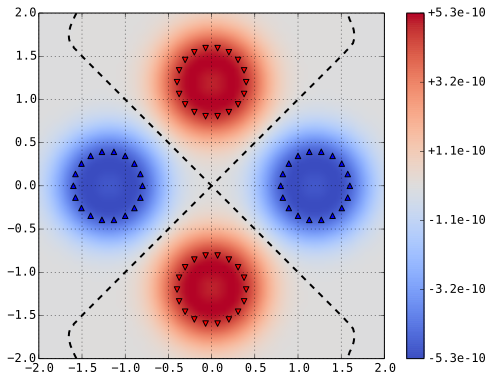
\includegraphics[width=.5\linewidth]{images/svm.kern1.eps}}
\subfloat[two concentric circles.]{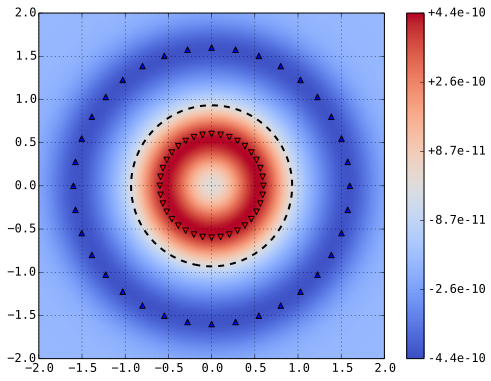
\includegraphics[width=.5\linewidth]{images/svm.kern2.eps}}
\caption{decision surface learned by a Gaussian SVM.\label{fig:svm:kern}}
\end{figure}

\sectref{smo}に掲載した実装に、適当な内積の定義を与えれば、任意の写像を試せる。手作りで、無限次元の魔法を味わおう。

\section{ヒルベルト空間}

\sectref{kernel}は、内積と距離が\eqref{kernel}の関数$k$で定義され、無限級数の極限も計算可能な空間$H_k$が存在する点に依拠する。
空間$H$が線型空間で、\eqref{kern:in}を満たす関数$\iprod{\bm{x}}{\bm{y}}$が存在する場合に、これを内積と呼び、空間$H$を\textbf{内積空間}と呼ぶ。
%
\begin{equation}
\label{eq:kern:in}
\forall a_i,b_j \in \mathbb{R} \colon
\iprod{\sum_{i=1}^I a_i \bm{x}_i}{\sum_{j=1}^J b_j \bm{y}_j} =
\iprod{\sum_{j=1}^J b_j \bm{y}_j}{\sum_{i=1}^I a_i \bm{x}_i} =
\sum_{i=1}^I \sum_{j=1}^J a_i b_j \iprod{\bm{x}_i}{\bm{y}_j},\esp
\iprod{\bm{x}}{\bm{x}} \geq 0.
\end{equation}
%
高校数学で学ぶ標準内積は、この定義に従う。また、関数$f,g$を元とする空間では、その内積は\eqref{kern:in:f}で定義できる。
%
\begin{equation}
\label{eq:kern:in:f}
\iprod{f}{g} = \int_H f(\bm{x}) \overline{g(\bm{x})} d\mu(\bm{x}).
\end{equation}
%
関数$\mu$は関数空間$H$の\textbf{測度}である。さて、内積空間$H$では、\eqref{kern:norm}に示す通り、内積を使って\textbf{ノルム}を定義できる。
%
\begin{equation}
\label{eq:kern:norm}
\norm{\bm{x}} = \iprod{\bm{x}}{\bm{x}}^{\FRAC{1}{2}} \in \mathbb{R}.
\end{equation}
%
\eqref{kern:norm}を利用して、任意の2点の距離$d$を定義できる。距離$d$が\eqref{knn:dist}を満たす場合に、空間$H$は\textbf{距離空間}である。
%
\begin{equation}
\label{eq:kern:dist}
d(\bm{x},\bm{y}) = \norm{\bm{x}-\bm{y}} \geq 0.
\end{equation}
%
空間$H$で定義された任意の級数が、空間$H$の元に収束する場合に、空間$H$は\textbf{完備性}を満たし、\textbf{ヒルベルト空間}となる。
正定値性を満たす適当な対称関数$k$を定義して、関数$k$の線型結合で\eqref{kern:H0}の空間$H_0$を作る。これを\textbf{線型包}と呼ぶ。
%
\begin{equation}
\label{eq:kern:H0}
H_0 = \mathrm{span}\seq{\sum_{n=1}^n a_n k(\bm{x}_n,\cdot)|a_n \in \mathbb{R}}.
\end{equation}
%
空間$H_0$の元$f,g$に対し、内積を\eqref{kern:in:H0}の通りに定義する。証明は省くが、空間$H_0$はヒルベルト空間の条件を満たす。
%
\begin{equation}
\label{eq:kern:in:H0}
\iprod{f}{g}_{H_0} = \sum_{i=1}^I \sum_{j=1}^J a_i b_j k(\bm{x}_i,\bm{x}_j),
\where
\left\{
\begin{aligned}
f(\bm{x}) &= \sum_{i=1}^I a_i k(\bm{x}_i,\bm{x}),\\
g(\bm{x}) &= \sum_{j=1}^J b_j k(\bm{x}_j,\bm{x}).
\end{aligned}
\right.
\end{equation}
%
ぜひ、\eqref{kern:in:H0}が\eqref{kern:in}の性質を満たし、その内積で距離$d$を定義すると、\eqref{knn:dist}の公理を満たす点を確認しよう。
さて、\eqref{kern:in:H0}より自明だが、空間$H_0$の元$f$は、\eqref{kern:reprod}の再生性を満たし、空間$H_0$は\textbf{再生核ヒルベルト空間}となる。
%
\begin{equation}
\label{eq:kern:reprod}
f(\bm{x}) = \sum_{n=1}^N a_n k(\bm{x}_n,\bm{x}) = \iprod{f}{k(\cdot,\bm{x})}_{H_0}.
\end{equation}
%
再生性を持つ関数$k$を\textbf{再生核}と呼ぶ。核は\eqref{kern:T}に示す\textbf{積分変換}に由来する。これは、空間$\Omega_s,\Omega_t$の間の写像である。
%
\begin{equation}
\label{eq:kern:T}
F(\bm{s}) = \int_{\Omega_t} k(\bm{s}, \bm{t}) f(\bm{t}) d\bm{t},
\where
\left\{
\begin{aligned}
\bm{s} &\in \Omega_s,\\
\bm{t} &\in \Omega_t.
\end{aligned}
\right.
\end{equation}
%
例えば、\textbf{ラプラス変換}や\textbf{フーリエ変換}が該当する。さて、\eqref{kern:rect}で定義される核関数$k$は、再生核である。証明しよう。
%
\begin{equation}
\label{eq:kern:sinc}
k(x,y) = \frac{a}{\pi} \sinc a(y-x).
\end{equation}
%
\eqref{kern:in:f}に従って内積を求めると、\eqref{kern:rect}を得る。\eqref{kern:sinc}が矩形関数の双対である点に注目して、再生性を導ける。
%
\begin{equation}
\label{eq:kern:rect}
\iprod{f}{k(x,\cdot)}_{L^2} =
\int_{-\infty}^\infty f(y) \overline{k(x,y)} dy =
\frac{1}{2\pi} \int_{-a}^a \mathcal{F}_f(\omega) e^{i \omega x} d\omega =
f(x).
\end{equation}
%
積分変換と機械学習の関係は興味深く、特に、深層学習の優れた性能の理由を積分変換に求める研究は、注目に値する。
簡単な例では、\eqref{kern:sigmoid}に示す\textbf{シグモイドカーネル}の挙動は、\eqref{nn:neuron}で加重$\bm{w}$が固定されたニューロンと等価になる。
%
\begin{equation}
\label{eq:kern:sigmoid}
k(\bm{w},\bm{x}) = \tanh \trans{\bm{w}} \bm{x}.
\end{equation}
%
深層学習は、勾配法を通じて加重$\bm{w}$を最適化するため、自在に最適化される高次元空間の層を持つのと等価だと言える。

\chapter{決定木の学習と汎化性能\label{chap:dt}}

意思決定の分野では、しばしば\textbf{決定木}と呼ばれる、質問と条件分岐の再帰的な木構造で、条件$\bm{x}$と結論$y$の関係を表す。
例えば、\eqref{dt:swim}は、海水浴の是非$y$を判断する決定木である。気象$\bm{x}$に対し、質問と条件分岐を繰り返し、結論を導く。
%
\begin{equation}
\label{eq:dt:swim}
y \approx f(\bm{x}) =
\begin{cases}
0 & \text{if $\mathrm{wavy}(\bm{x}) = 1$} \\
\text{otherwise}
\left\{
\begin{aligned}
& 0 && \text{if $\mathrm{rain}(\bm{x}) = 1$} \\
& 1 && \text{if $\mathrm{rain}(\bm{x}) = 0$} \\
\end{aligned}
\right\}
& \text{if $\mathrm{wavy}(\bm{x}) = 0$} \\
\end{cases}
\end{equation}
%
決定木の学習では、意思決定の事例の集合$\seqXy$に対し、簡潔で解釈の容易な質問と条件分岐と、その順序を習得する。

\section{情報源符号化定理\label{sect:info}}

理想的な決定木は、簡潔明瞭である。即ち、最低限の質問で、結論に至る。ここで、\textbf{情報源符号化}の概念を導入しよう。
質問と条件分岐を繰り返す過程は、条件$\bm{x}$の情報を分解し、情報の断片に2進数の\textbf{符号語}を割り振る操作と等価である。
%
\begin{equation}
C(\bm{x}) \colon \bm{x} \mapsto \bm{s} \in \seq{0, 10, 11}.
\end{equation}
%
事象$\bm{x}$が従う確率分布$\prob{\bm{x}}$を仮定して、事象$\bm{x}$が伴う情報の価値$I(\bm{x})$を定義する。質問の妥当性に相当する量である。
情報の価値とは、その事象の希少性である。即ち、価値$I(\bm{x})$は、確率$\prob{\bm{x}}$に対して単調減少であり、\eqref{dt:info:rare}を満たす。
%
\begin{equation}
\label{eq:dt:info:rare}
\prob{\bm{x}_i} \leq \prob{\bm{x}_j} \Leftrightarrow I(\bm{x}_i) \geq I(\bm{x}_j).
\end{equation}
%
また、複数の事象が同時に発生した場合の情報の価値は、個別に発生した場合の情報の価値の総和となると自然である。
%
\begin{equation}
\label{eq:dt:info:add}
I(\bm{x}_1,\bm{x}_2,\ldots,\bm{x}_N) = \sum_{n=1}^N I(\bm{x}_n).
\end{equation}
%
\eqref{dt:info:add}の性質を\textbf{情報の加法性}と呼ぶ。以上の性質を満たす定義を考えると、\eqref{dt:info}を得る。この$I(\bm{x})$を\textbf{情報量}と呼ぶ。
%
\begin{equation}
\label{eq:dt:info}
I(\bm{x}) = \log_2 \frac{1}{\prob{\bm{x}}} = - \log_2 \prob{\bm{y}} \geq 0.
\end{equation}
%
符号$C$の符号語を圧縮するには、事象$\bm{x}$に、情報量に応じた長さの符号語を割り振る。これを\textbf{エントロピー符号}と呼ぶ。
符号語の長さの期待値$\overline{L}$は、\eqref{dt:shannon}の\textbf{シャノンの情報源符号化定理}に従う。関数$H$を確率分布$p$の\textbf{平均情報量}と呼ぶ。
%
\begin{equation}
\label{eq:dt:shannon}
\overline{L(C)} \geq H(p) = \sum_{\bm{x}} \prob{\bm{x}} I(\bm{x}) = -\sum_{\bm{x}} \prob{\bm{x}} \log_2 \prob{\bm{x}} \geq 0.
\end{equation}
%
情報量の議論を利用して、質問の回数を圧縮する方法を検討しよう。まず、最初の質問は、情報量が最大の質問を選ぶ。
質問$Q$により、集合$X$が$K$通りの部分集合$X_k$に分割される場合は、質問$Q$の情報量$G(Q)$は、\eqref{dt:gain}で定義される。
%
\begin{equation}
\label{eq:dt:gain}
G(Q) = H(X) - H(X|Q) = H(X) - \sum_{k=0}^{K-1} \Prob{X_k}[X] H(X_k) \geq 0.
\end{equation}
%
同様に、部分集合$X_k$に対し、情報量が最大の質問を選び、次の質問とする。この操作を繰り返し、最適な決定木を得る。
質問の回数は整数なので、決定木が表す分布$\hatp$は、分布$p$と異なる。その様子を表す$H(p,\hatp)$を\textbf{交差エントロピー}と呼ぶ。
%
\begin{equation}
\label{eq:dt:KL}
\overline{L(C)} = H(p,q) =
-\sum_{\bm{x}} \prob{\bm{x}} \log \hatprob{\bm{x}} =
-\sum_{\bm{x}} \prob{\bm{x}} \left\{\log \prob{\bm{x}} - \log\frac{\prob{\bm{x}}}{\hatprob{\bm{x}}}\right\} =
H(p) + \KL{p}{q} \geq H(p).
\end{equation}
%
余分な質問の回数を表す$\KL{p}{\hatp}$を\textbf{カルバック・ライブラー情報量}と呼ぶ。これは、確率分布$p,\hatp$の差を表す量でもある。

\section{条件分岐の最適化}

\sectref{info}の議論に基づき、決定木を実装する。まず、推論を抽象化する。条件$\bm{x}$は整数の列で、結論$y$は任意の型とする。

\begin{Verbatim}{Scala}
trait Node[T] extends (Seq[Int] => T)
\end{Verbatim}

次に、決定木の本体を実装する。引数は、決定木が学習する集合$\seqXy$と、決定木の末端の細分化を抑える閾値である。
決定木は再帰的に生成されるが、質問の情報量が微小の場合は、分布$\prob{y}$の最大値を与える$y$を定数値として出力する。

\begin{Verbatim}{Scala}
case class Question[T](x: Seq[(Seq[Int], T)], limit: Double = 1e-5) extends Node[T] {
	lazy val m = x.groupBy(_._2).maxBy(_._2.size)._1
	lazy val p = x.groupBy(_._2).map(_._2.size.toDouble / x.size)
	lazy val ent = p.map(p => -p * math.log(p)).sum / math.log(2)
	lazy val division = x.head._1.indices.map(split).minBy(_.ent)
	def apply(x: Seq[Int]) = if(ent - division.ent < limit) m else division(x)
	def split(v: Int) = x.map(_._1(v)).toSet.map(Division(x,v,_)).minBy(_.ent)
}
\end{Verbatim}

次に、条件分岐を実装する。引数は、決定木が学習する集合$\seqXy$と、条件$\bm{x}$を分割する軸と、分割を行う閾値である。
分割する軸と値は、\eqref{dt:gain}で議論した通り、質問の情報量を最大化する軸と値が選択される。これで決定木が完成した。

\begin{Verbatim}{Scala}
case class Division[T](x: Seq[(Seq[Int], T)], axis: Int, value: Int) extends Node[T] {
	val sn1 = Question(x.filter(_._1(axis) >  value))
	val sn2 = Question(x.filter(_._1(axis) <= value))
	val ent = (sn1.ent * sn1.x.size + sn2.ent * sn2.x.size) / x.size
	def apply(x: Seq[Int]) = if(x(axis) >= value) sn1(x) else sn2(x)
}
\end{Verbatim}

\figref{dt:plain}は、各々が正規分布に従う3クラスの点の集合を学習し、決定木で空間をそれらのクラスに分割した結果である。
結果的に、過剰に複雑な境界となった。個別の事例には忠実だが、正規分布の形からは乖離した。これを\textbf{過学習}と呼ぶ。

\begin{figure}[h]
\centering
\subfloat[$\mathtt{limit}=1e-5$.\label{fig:dt:plain:abs}]{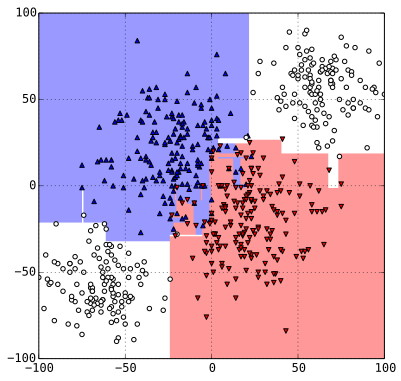
\includegraphics[width=.5\linewidth]{images/id3.plain.eps}}
\subfloat[$\mathtt{limit}=1e-1$.\label{fig:dt:plain:sup}]{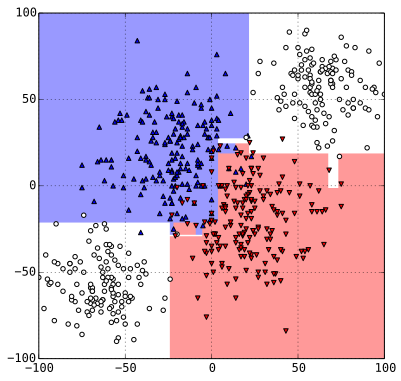
\includegraphics[width=.5\linewidth]{images/id3.prune.eps}}
\caption{region segmentation by a decision tree.\label{fig:dt:plain}}
\end{figure}

過学習は、機械学習で普遍的な課題だが、特に、決定木は、際限なく細分化できるため、しばしば表現能力が過剰である。
過学習を抑えるには、\subfigref{dt:plain}{sup}のように、分割の閾値を調節するか、\sectref{dt:ensem}で学ぶ\textbf{アンサンブル学習}が有効である。

\section{アンサンブル学習\label{sect:dt:ensem}}

決定木に限らず、機械学習では、真の関係$f$と、習得した関係$\hat{f}$の間に若干の差があり、それが過学習として顕在化する。
過学習の原因は、教師データの偏りや、関数$\hat{f}$の過剰な表現能力にある。関数$f,\hat{f}$の差を2乗誤差関数で定式化しよう。
%
\begin{equation}
\label{eq:dt:bag:E}
\int_{\bm{x}}\prob{\bm{x}}(y-\hat{f}(\bm{x}))^2d\bm{x} = \Var{y-f(\bm{x})} + \tup{\E{\hat{f}(\bm{x})} - f(\bm{x})}^2 + \Var{\hat{f}(\bm{x})}.
\end{equation}
%
\eqref{dt:bag:E}の第2項の平方根を\textbf{バイアス}と、第3項を\textbf{バリアンス}と呼ぶ。この2項が過学習や、逆に学習不足の原因となる。
両者はトレードオフの関係にあるが、$T$個の関数$\hat{f}_t$を\textbf{弱学習器}とし、投票を行う\textbf{アンサンブル学習}により、調節できる。
%
\begin{equation}
\label{eq:dt:bag:f}
\hat{f}(\bm{x}) = \frac{1}{T} \sum_{t=1}^T \hat{f}_t(\bm{x}).
\end{equation}
%
過学習を防ぐには、相互に独立した弱学習器の訓練が重要である。そこで、事例を選び直す\textbf{ブートストラップ法}を行う。
要素の重複を許して$T$通りの部分集合を作成し、$T$通りの弱学習器$f_t$を訓練する。これで、\eqref{dt:bag:C}の分散が低減する。
%
\begin{equation}
\label{eq:dt:bag:C}
\Var{\hat{f}(\bm{x})} = \frac{1}{T^2}\sum_{i=1}^T \sum_{j=1}^T \Cov{f_i(\bm{x}),f_j(\bm{x})}.
\end{equation}
%
この手法は\textbf{バギング}とも呼ばれる。基本的には、決定木や深層学習など表現能力が過剰な手法に使う。以下に実装する。

\begin{Verbatim}{Scala}
case class Bagging[T](x: Seq[(Seq[Int], T)], t: Int, n: Int) extends Node[T] {
	val f = Seq.fill(t)(Question(Seq.fill(n)(x(util.Random.nextInt(x.size)))))
	def apply(x: Seq[Int]) = f.map(_(x)).groupBy(identity).maxBy(_._2.size)._1
}
\end{Verbatim}

\section{ブースティング法}

逆に、学習不足の解消には、弱学習器の表現能力を補う弱学習器を作り、加重投票を行う\textbf{ブースティング法}を適用する。
%
\begin{equation}
\hat{f}(\bm{x}) = \sum_{t=1}^T w_t \hat{f}_t(\bm{x}).
\end{equation}
%
弱学習器$f_t$は、弱学習器$f_1,\ldots,f_{t-1}$が判断を誤った点$\bm{x}$を重点的に学習する。点$\bm{x}$を選ぶ確率分布$q_t(\bm{x})$を検討しよう。
分類問題を想定し、\eqref{dt:ada:E}に示す\textbf{指数誤差}を最小化する。指数誤差の最小化は、関数$\bm{f},\hat{\bm{f}}$の値の内積の最大化である。
%
\begin{equation}
\label{eq:dt:ada:E}
E(\hat{\bm{f}}) =
\exp \seq{-\trans{\bm{f}(\bm{x})} \hat{\bm{f}}(\bm{x})} =
\exp \seq{-\trans{\bm{f}(\bm{x})} \sum_{t=1}^T w_t \hat{\bm{f}}_t(\bm{x})} \geq 0.
\end{equation}
%
次に、特に分類問題を想定し、関数$\hat{\bm{f}}$が取り得る値に制約条件を設定する。関数$\bm{f},\hat{\bm{f}}$の値は、\eqref{dt:ada:sum}の条件を満たす。
%
\begin{equation}
\label{eq:dt:ada:sum}
\sum_{k=1}^K f(\bm{x},k) =
\sum_{k=1}^K \hat{f}(\bm{x},k) = 1,
\where
\left\{
\begin{aligned}
\bm{f}(\bm{x}) =
\begin{bmatrix}
f(\bm{x},k)
\end{bmatrix}_k,\\
\hat{\bm{f}}(\bm{x}) =
\begin{bmatrix}
\hat{f}(\bm{x},k)
\end{bmatrix}_k.
\end{aligned}
\right.
\end{equation}
%
具体的には、真の関数$\bm{f}$は、\eqref{dt:ada:f}に示す値を取る。ただし、関数$\hat{\bm{f}}$は、\eqref{dt:ada:sum}を満たす範囲で、自由な値を取る。
%
\begin{equation}
\label{eq:dt:ada:f}
f(\bm{x},k) =
\begin{cases}
\hfil1\hfil& \text{if $y=k$},\\
\frac{1}{1-K}& \text{if $y\neq k$}.
\end{cases}
\end{equation}
%
\eqref{dt:ada:E}を分解すると、\eqref{dt:ada}を得る。この関数$q_T$を確率分布として、弱学習器$f_T$が学習する集合を無作為に選ぶ。
%
\begin{equation}
\label{eq:dt:ada}
E(\hat{\bm{f}}) =
q_T(\bm{x}) \exp \seq{-\bm{f}(\bm{x}) w_T \hat{\bm{f}}_T(\bm{x})},
\where
q_T(\bm{x}) =
\exp \seq{-\bm{f}(\bm{x}) \sum_{t=1}^{T-1} w_t \hat{\bm{f}}_t(\bm{x})}.
\end{equation}
%
弱学習器$f_T$に対し、指数誤差$E$を最小化する加重$w_T$は、\eqref{dt:ada:w}で計算できる。\textbf{ラグランジュの未定乗数法}を使った。
%
\begin{equation}
\label{eq:dt:ada:w}
\hat{w}_T = \log \tup{\frac{1-E_T}{E_T}} + \log (K-1),
\where
E_T = q_T(\bm{x},y) \mathbb{I}(\hat{f}_T(\bm{x}) \neq y).
\end{equation}
%
以上の手法は、\textit{AdaBoost}と呼ばれる。他にも、弱学習器の誤差を別の弱学習器で補う、\textbf{勾配ブースティング}が存在する。

\section{汎化性能の最適化}

\sectref{dt:ensem}の議論を踏まえ、\textit{AdaBoost}を実装しよう。基本的には、弱学習器を逐次的に作成し、追加する操作を繰り返す。

\begin{Verbatim}{Scala}
case class AdaBoost[T](x: Seq[(Seq[Int], T)], m: Int) extends Node[T] {
	val k = x.map(_._2).toSet
	val t = Seq(AdaStage(x, Seq.fill(x.size)(1.0 / x.size), m)).toBuffer
	def apply(x: Seq[Int]) = k.maxBy(y => t.map(_.score(x, y)).sum)
	while(t.last.best.error < 0.5) t += AdaStage(x, t.last.next, m)
}
\end{Verbatim}

弱学習器$f_t$は、$M$個の候補$\hat{f}_{tm}$を作成し、最も高精度な候補を$f_t$とする。この操作を$E_t$が$0.5$を超えるまで繰り返す。

\begin{Verbatim}{Scala}
case class AdaStage[T](x: Seq[(Seq[Int], T)], p: Seq[Double], m: Int) extends Node[T] {
	val best = List.fill(m)(Resample(x, p.map(_ / p.sum))).minBy(_.error)
	val gain = math.log((1 / best.error - 1) * (x.map(_._2).toSet.size - 1))
	val next = x.map(score).map(gain - _).map(math.exp).zip(p).map(_ * _)
	def score(x: Seq[Int], y: T) = if(this(x) == y) gain else 0
	def apply(x: Seq[Int]) = best(x)
}
\end{Verbatim}

弱学習器の候補$\hat{f}_{tm}$は、確率分布$q_t$に従う部分集合$\TRAIN_t$を学習する。集合$\TRAIN_t$は\textbf{ノイマンの棄却法}で擬似的に抽出できる。

\begin{Verbatim}{Scala}
case class Resample[T](x: Seq[(Seq[Int], T)], p: Seq[Double]) extends Node[T] {
	val data = Seq[(Seq[Int], T)]().toBuffer
	def reject(i: Int) = if(util.Random.nextDouble * p.max < p(i)) x(i) else null
	while(data.size < p.size) data += reject(util.Random.nextInt(p.size)) -= null
	def error = x.map((x, y) => this(x) != y).zip(p).filter(_._1).map(_._2).sum
	def apply(x: Seq[Int]) = quest(x)
	val quest = Question(data.toList)
}
\end{Verbatim}

\figref{dt:ensem}は、各々が正規分布に従う3クラスの事例を学習した結果である。比較のため、\figref{dt:plain}と同じ事例を使用した。

\begin{figure}[h]
\centering
\subfloat[\texttt{Bagging}  class.]{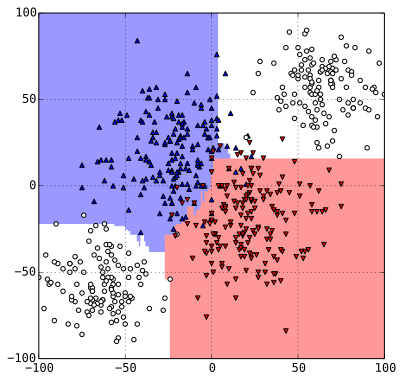
\includegraphics[width=.5\linewidth]{images/id3.bag50.eps}}
\subfloat[\texttt{AdaBoost} class.]{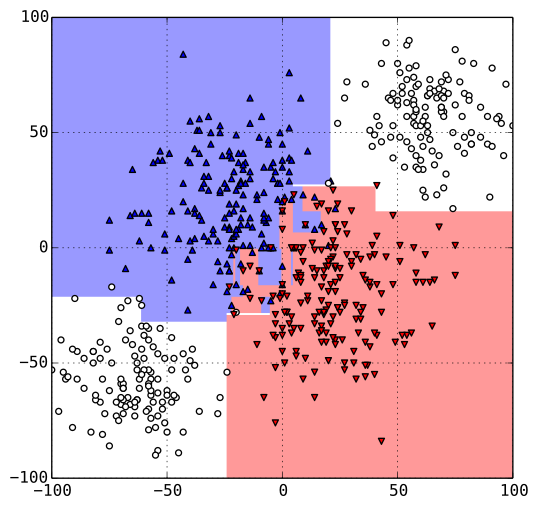
\includegraphics[width=.5\linewidth]{images/id3.ada50.eps}}
\caption{region segmentation by ensemble learning.\label{fig:dt:ensem}}
\end{figure}

決定木は、表現能力が過剰なので、学習不足を補うブースティングより、過学習を抑えるバギングの方が効果的である。

\section{圧縮アルゴリズム\label{sect:huff}}

\sectref{info}で学んだ情報源符号化は、機械学習よりも、可逆圧縮の理論として知られる。その代表例が\textbf{ハフマン符号}である。
決定木に似た\textbf{ハフマン木}を作り、その分岐に2進数の符号語を割り当て、再帰的に圧縮と復元を行う。以下に実装を示す。

\begin{Verbatim}{Scala}
abstract class Node(val s: String, val w: Int) {
	def decode(bits: String, root: Node = this): String
	def encode(text: String, root: Node = this): String
}
\end{Verbatim}

引数は、この頂点が表す文字と、文字が現れる頻度である。また、文字列を受け取り、圧縮と復元を行う機能を実装する。
以下に、末端の頂点を実装する。復元の際は、頂点に対応する文字を出力し、圧縮の際は、何もせず最上位の頂点に戻る。

\begin{Verbatim}{Scala}
case class Atom(ch: String, freq: Int) extends Node(ch, freq) {
	def decode(bits: String, root: Node) = if(bits.isEmpty) ch else ch ++ root.decode(bits, root)
	def encode(text: String, root: Node) = if(text.size < 2) "" else root.encode(text.tail, root)
}
\end{Verbatim}

次に、符号語を表す頂点を実装する。厳密には、頂点と符号語の1桁を紐付けた頂点で、圧縮の際に、その桁を出力する。

\begin{Verbatim}{Scala}
case class Code(node: Node, bit: String) extends Node(node.s, node.w) {
	def decode(bits: String, root: Node) = node.decode(bits.tail, root)
	def encode(text: String, root: Node) = bit++node.encode(text, root)
}
\end{Verbatim}

分岐も実装する。復元の際は、符号語の$0,1$に対応する頂点を、圧縮の際は、圧縮する文字を含む頂点を選び、巡回する。

\begin{Verbatim}{Scala}
case class Fork(nodes: Seq[Code]) extends Node(nodes.map(_.s).mkString, nodes.map(_.w).sum) {
	def decode(bits: String, root: Node) = nodes.find(_.bit.head == bits.head).get.decode(bits, root)
	def encode(text: String, root: Node) = nodes.find(_.s.contains(text.head)).get.encode(text, root)
}
\end{Verbatim}

次に、再帰的に木構造を構築する手順を実装する。まず、頻度が最低の部分木の組を選び、その親となる分岐を構築する。
また、部分木の頻度を合計し、新たな部分木の頻度とする。この操作を逐次的に繰り返し、完全なハフマン木を構築する。

\begin{Verbatim}{Scala}
implicit class Huffman(nodes: Seq[Node]) {
	def fork: Seq[Code] = nodes.zipWithIndex.map(_->_.toString).map(Code(_,_))
	def join: Seq[Node] = Seq(Fork(nodes.take(2).fork)).union(nodes.tail.tail)
	def tree: Seq[Node] = if(nodes.size <= 1) nodes else join.sortBy(_.w).tree
}
\end{Verbatim}

最後に、暗黙の型変換を利用して、文字列からハフマン木を生成する機能も実装した。この文字列が、圧縮の対象となる。

\begin{Verbatim}{Scala}
implicit class Symbols(source: String) {
	def countFreq = source.split("").groupBy(identity).mapValues(_.size)
	def toHuffman = countFreq.toSeq.map(Atom(_,_)).sortBy(_.w).tree.head
}
\end{Verbatim}

以上で、可逆圧縮が完成した。以下に、使用例を示す。なお、未知の文字を圧縮すると、例外が発生する点に、注意する。

\begin{Verbatim}{Scala}
val encoded = "Lorem ipsum dolor sit amet consectetur adipiscing elit".toHuffman.encode("lorem")
val decoded = "Lorem ipsum dolor sit amet consectetur adipiscing elit".toHuffman.decode(encoded)
println(encoded)
println(decoded)
\end{Verbatim}

以下に、出力を示す。文字が出現する頻度の偏りに起因して、平均情報量が抑制されたため、半分の圧縮率を達成できた。

\begin{Verbatim}{bash}
110011110010100011111
lorem
\end{Verbatim}

\chapter{潜在的ディリクレ配分法\label{chap:lda}}

自然言語の機械学習には、特有の困難がある。特定の形態素が出現する確率は低く、その確率も話題に応じて変化する。
話題も曖昧で多岐に渡り、教師あり学習が困難なので、単語$w$の背後にある話題$z$を、教師なし学習する方法を考える。

\section{確率的潜在意味解析\label{sect:lda}}

話題$z$は観測できず、潜在的な情報である。また、話題$z$の分布は、記事の主題に応じて変化する。その点を考慮しよう。
具体的には、単語$w$の出現が、試行1回の\textbf{多項分布}に従うと考える。また、単語$w$と話題$z$が従う確率分布を仮定する。
%
\begin{equation}
\label{eq:lda}
\Prob{w,z,\phi,\theta} =
\Prob{w}[\phi] \Prob{\phi} \Prob{z}[\theta] \Prob{\theta} =
\tup{\prod_{v=1}^V \phi_{zv}^{N_v}} \Dd{\phi}{\nu} \tup{\prod_{k=1}^K \theta_k^{N_k}} \Dd{\theta}{\alpha}.
\end{equation}
%
変数$N_v,N_k$は、単語$v$と話題$k$の出現の数で、総和は$1$である。変数$\phi_v,\theta_k$は、単語$v$と話題$k$が出現する確率である。
\eqref{lda:mul}の多項分布は、話題$k$が確率$\theta_k$で現れる記事から$N$語を取得して、話題$k$の単語が$N_k$個となる確率を与える。
%
\begin{equation}
\label{eq:lda:mul}
\Prob{z}[\theta] =
N! \prod_{k=1}^K \frac{\theta_k^{N_k}}{N_k!},
\where
\sum_{k=1}^K N_k = N.
\end{equation}
%
\eqref{lda:dir}の\textbf{ディリクレ分布}は、話題$k$の単語が$N_k-1$個だった場合に、実際に話題$k$が確率$\theta_k$で出現する確率を与える。
これは、変数$N$を連続量に拡張した多項分布である。\eqref{lda:dir}に従う話題$z$の推定を、\textbf{潜在的ディリクレ配分法}と呼ぶ。
%
\begin{equation}
\label{eq:lda:dir}
\Prob{\theta} =
\Dd{\theta}{N} =
\Gd{\sum_{k=1}^K N_k} \prod_{k=1}^K \frac{\theta_k^{N_k-1}}{\Gd{N_k}} =
\frac{1}{\Bd{N}} \prod_{k=1}^K \theta_k^{N_k-1}.
\end{equation}
%
\eqref{lda:dir}で、関数$\Gp$は\textbf{ガンマ関数}で、自然数の階乗$(n-1)!$を複素数の階乗に拡張した関数である。\eqref{lda:gamma}に定義する。
%
\begin{equation}
\label{eq:lda:gamma}
\Gd{n} = \int_0^{\infty} x^{n-1} e^{-x} dx.
\end{equation}
%
関数$\Bp$は\textbf{ベータ関数}を多変量に拡張した複素関数で、\eqref{lda:mul}に現れる多項係数の逆数に相当する。\eqref{lda:beta}が成立する。
%
\begin{equation}
\label{eq:lda:beta}
\Bd{N} =
\int \prod_{k=1}^K x_k^{N_k+1} d\bm{x} =
\idotsint \prod_{k=1}^K x_k^{N_k+1} dx_1 dx_2 \cdots dx_K,
\where
\sum_{k=1}^K x_k = 1.
\end{equation}
%
\eqref{lda:beta}から、\eqref{lda:z}が簡単に導ける。\eqref{lda:z}の性質は、確率$\theta$を実際の記事から推定する際に、重要な役割を果たす。
%
\begin{equation}
\label{eq:lda:z}
\Prob{z} =
\int \Prob{z}[\theta] \Prob{\theta} d\bm{\theta} =
N! \frac{\Bd{\hat{\alpha}}}{\Bd{\alpha}} \prod_{k=1}^K \frac{1}{N_k!},
\where
\hat{\alpha}_k = \alpha_k + N_k.
\end{equation}
%
記事を学習すると、確率$\theta_k$の最適値は\eqref{lda:post}に従う。これを事後確率と呼ぶ。また、\eqref{lda:mul}を確率$\theta_k$の尤度と呼ぶ。
学習前では、どの話題の出現も均等と仮定し、\eqref{lda:dir}に従って、確率$\theta_k$に初期値を設定できる。これを事前確率と呼ぶ。
%
\begin{equation}
\label{eq:lda:post}
\theta_k \sim
\Prob{\theta}[z] =
\frac{\Prob{z}[\theta] \Prob{\theta}}{\Prob{z}} =
\frac{1}{\Bd{\hat{\alpha}}} \prod_{k=1}^K \theta_k^{\hat{\alpha}_k-1}.
\end{equation}
%
\eqref{lda:post}は、観測を重視して、尤度を最適化する最尤推定と対照的で、観測の偏りを重視する。これを\textbf{ベイズ推定}と呼ぶ。
最尤推定では、観測の偏りに起因した過学習が発生するが、その点が解消される。さて、\eqref{lda:beta}から\eqref{lda:gibbs}が導ける。
%
\begin{equation}
\label{eq:lda:gibbs}
\E{\theta_k} \E{\phi_{kv}} =
\frac{\hat{\alpha}_k}{\norm{\hat{\alpha}}_1}
\frac{\hat{\nu}_{kv}}{\norm{\hat{\nu}_k}_1},
\where
\norm{\hat{\alpha}}_1 = \sum_{k=1}^K \alpha_k,\esp
\norm{\hat{\nu}_k}_1 = \sum_{v=1}^V \nu_{kv}.
\end{equation}
%
\eqref{lda:gibbs}に従う乱数により、変数$z$を何度も選び直すと、最終的に真の分布$\theta$に収束する。これを\textbf{モンテカルロ法}と呼ぶ。
\chapref{gmm}で学ぶ変分ベイズ法と比較して、収束に時間を要するが、複雑な確率分布にも適用でき、並列処理も容易である。

\section{潜在的な話題の学習}

\sectref{lda}の潜在的ディリクレ配分法を実装する。まず、単語と話題の組$\pair{w}{z}$を実装する。話題$z$は無作為に初期化する。

\begin{Verbatim}{scala}
case class Word[W](v: W, k: Int) {
	var z = util.Random.nextInt(k)
}
\end{Verbatim}

潜在的ディリクレ配分法の本体を実装する。引数は、記事と単語の集合に、話題の総数と、母数$\alpha,\nu$の初期値を与える。

\begin{Verbatim}{scala}
class LDA[D,W](texts: Map[D,Seq[W]], val k: Int, a: Double = 0.1, n: Double = 0.01) {
	val words = texts.map(_ -> _.map(Word(_,k)))
	val vocab = words.flatMap(_._2).groupBy(_.v)
	val nd = words.map((d,s) => d -> Array.tabulate(k)(k => s.count(_.z == k) + a)).toMap
	val nv = vocab.map((v,s) => v -> Array.tabulate(k)(k => s.count(_.z == k) + n)).toMap
	val nk = Array.tabulate(k)(k => nv.map(_._2(k)).sum)
	def apply(k: Int) = vocab.keys.toList.filter(v => nv(v).max == nv(v)(k))
	def probs(v: W, d: D) = 0.until(k).map(k => nv(v)(k) * nd(d)(k) / nk(k))
}
\end{Verbatim}

以上の実装を継承して、モンテカルロ法を実装する。まず、適当な組$\pair{w}{z}$を選び、その分を変数$\alpha_z,\nu_z$から除去する。
次に、\eqref{lda:gibbs}に従う乱数を\textbf{ノイマンの棄却法}で生成し、話題$z$を選び直し、母数$\alpha_z,\nu_z$に加える。この手順を繰り返す。

\begin{Verbatim}{scala}
class Gibbs[D,W](texts: Map[D,Seq[W]], k: Int, epochs: Int = 500) extends LDA(texts, k) {
	for(epoch <- 1 to epochs; (document,words) <- util.Random.shuffle(words); w <- words) {
		nk(w.z) -= 1
		nv(w.v)(w.z) -= 1
		nd(document)(w.z) -= 1
		val uni = util.Random.between(0, probs(w.v,document).sum.toDouble)
		w.z = probs(w.v,document).scan(0.0)(_+_).tail.indexWhere(_ >= uni)
		nd(document)(w.z) += 1
		nv(w.v)(w.z) += 1
		nk(w.z) += 1
	}
}
\end{Verbatim}

以上で完成した。使用例を示す。これは、素数$k$を話題と、その倍数を単語と見做し、無作為に生成した数列を学習する。
単語$v$の共起と、記事毎に異なる話題の分布を再現した。学習が進むと、同じ約数を持つ整数が、同じ話題に分配される。

\begin{Verbatim}{scala}
val bases = Seq(2,3,5,7,11)
def sample(n: Int, m: Int, k: Int) = Seq.fill(n)(k * util.Random.nextInt(m / k + 1)) 
val texts = Seq.fill(1000)(bases.map(sample(util.Random.nextInt(100),50,_)).flatten)
val gibbs = new Gibbs(texts.indices.zip(texts).toMap, bases.size)
\end{Verbatim}

\section{単語の類似度の推定}

確率$\phi$を単語の意味を表す変数と考え、その距離に従って、単語を分類しよう。\chapref{gmm}で実装する\kmean{}を利用する。

\begin{Verbatim}{Scala}
val kmeans = new Kmeans(gibbs.nv.values.map(_.toList).toSeq, gibbs.k)
val topics = texts.flatten.distinct.topicBy(v => kmeans(gibbs.nv(v)))
for(topic <- topics.values) println(topic.toSeq.sorted.mkString(","))
\end{Verbatim}

以下に、出力を示す。共通の約数を持つ自然数が綺麗に分離できた。共起に基づく確率的な話題推定の有効性が窺える。

\begin{Verbatim}{bash}
0,7,14,21,28,35,42,49,56,63,70,77
5,10,15,20,25,30,40,45,50,55,60,65,75,80
3,6,9,12,18,24,27,33,36,39,48,51,54,57,66,69,72,78
2,4,8,16,22,26,32,34,38,44,46,52,58,62,64,68,74,76
\end{Verbatim}

\chapter{混合正規分布と最尤推定\label{chap:gmm}}

適当な観測量$\bm{x}$から、それが従う確率分布$p$を推定する手法が最尤推定である。具体的には、分布$p$の母数を推定する。
%
\begin{equation}
\forall\bm{x}\colon \bm{x} =
\begin{pmatrix}
x_1\\
x_2\\
\vdots\\
x_D
\end{pmatrix}
\sim \prob{\bm{x}}.
\end{equation}
%
例えば、正規分布$\mathcal{N}$を仮定する場合は、平均$\bm{\mu}$と分散$S$が母数に該当する。ただし、分散$S$とは分散共分散行列を指す。
%
\begin{equation}
\label{eq:gmm:n}
\Nd{\bm{x}}{\bm{\mu},S} =
\frac{1}{\Nn{S}} \exp \seq{-\frac{1}{2} \trans{(\bm{x}-\bm{\mu})} S^{-1} (\bm{x}-\bm{\mu})},
\where
\Nn{S} = \sqrt{(2\pi)^D\abs{S}}.
\end{equation}
%
正規分布では簡単なので、複数の正規分布の線型和を考えよう。\eqref{gmm}を\textbf{混合正規分布}と呼ぶ。定数$w_k$は加重である。
%
\begin{equation}
\label{eq:gmm}
\bm{x} \sim \prob{\bm{x}} = \sum_{k=1}^K w_k \Nd{\bm{x}}{\bm{\mu}_k,S_k},
\where
\sum_{k=1}^K w_k = 1.
\end{equation}
%
正規分布を点$\bm{x}$の集団または\textbf{クラスタ}と見做せば、混合正規分布の最尤推定は、点$\bm{x}$が属す集団$C_k$の推定と同義である。
%
\begin{equation}
\Prob{\bm{x} \in C_k} =
\frac{\Prob{C_k}\Prob{\bm{x}}[C_k]}{\Prob{\bm{x}}} =
\frac{w_k \Nd{\bm{x}}{\bm{\mu}_k,S_k}}{\prob{\bm{x}}}.
\end{equation}
%
点$\bm{x}$がどの集団$C_k$に属すかは観測できず、潜在的な情報である。この情報を変数$z$で表すと、変数$z$は潜在変数となる。
\figref{gmm}は、混合正規分布の例である。\eqref{gmm}の母数を推定し、点$\bm{x}$で支配的な集団を求めれば、点$\bm{x}$の帰属がわかる。

\begin{figure}[h]
\centering
\subfloat[cluster map.\label{fig:gmm:class}]{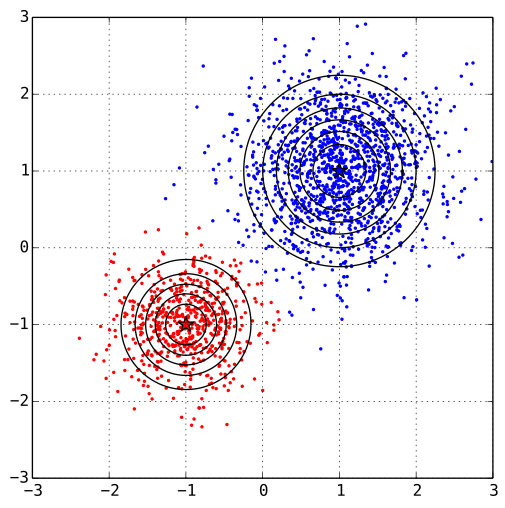
\includegraphics[width=.5\linewidth]{images/gmm.truth.eps}}
\subfloat[density map.\label{fig:gmm:dense}]{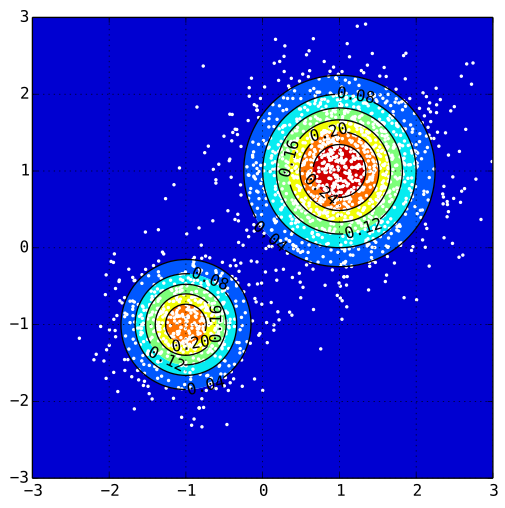
\includegraphics[width=.5\linewidth]{images/gmm.dense.eps}}
\caption{Ground-truth data of a Gaussian mixture model.\label{fig:gmm}}
\end{figure}

\subfigref{gmm}{class}の分類問題を、\textbf{クラスタリング}と呼ぶ。推定対象の値が潜在変数な点を指して、教師なし学習とも呼ばれる。

\section{クラスタリングの実装\label{sect:km}}

\sectref{km}では、混合正規分布や最尤推定の議論は忘れて、集合を最適なクラスタに分割する、素朴な方法を検討しよう。
理想的な集合$C_k$では、その要素$\bm{x}$と、集合$C_k$の重心$\bm{\mu}_k$の距離が最短となる。この命題を定式化して、\eqref{km:D}を得る。
%
\begin{equation}
\label{eq:km:D}
\min \mathcal{D} =
\min \sum_{n=1}^N \sum_{k=1}^K z_{nk} \norm{\bm{x}_n-\bm{\mu}_k}^2,
\where
\hat{z}_{nk} =
\begin{cases}
1,& \text{if $\bm{x}_n     \in C_k$},\\
0,& \text{if $\bm{x}_n \not\in C_k$}.
\end{cases}
\end{equation}
%
\eqref{km:D}の最適化は、逐次的に行う。まず、重心$\bm{\mu}_k$を乱数で初期化する。次に、\eqref{km:Z}に従って、変数$z_{nk}$を修正する。
%
\begin{equation}
\label{eq:km:Z}
\hat{z}_{nk} =
\begin{cases}
1,& \text{if $k=   \argmin_j\norm{\bm{x}_n-\bm{\mu}_j}^2$},\\
0,& \text{if $k\neq\argmin_j\norm{\bm{x}_n-\bm{\mu}_j}^2$}.
\end{cases}
\end{equation}
%
最後に、\eqref{km:M}により、重心$\bm{\mu}_k$を修正する。\eqref{km:M}は、変数$z_{nk}$を固定して、\eqref{km:D}を重心$\bm{\mu}_k$で微分すると導ける。
%
\begin{equation}
\label{eq:km:M}
\hat{\bm{\mu}}_k = \frac{1}{N_k} \sum_{n=1}^N z_{nk} \bm{x}_n,
\where
N_k = \sum_{n=1}^N z_{nk},
\Leftarrow
\pdiff{\mathcal{D}}{\bm{\mu}_k} = 0.
\end{equation}
%
以上の手順を繰り返し、最適解を得る。この手法を\kmean{}と呼ぶ。混合正規分布を仮定した考察は、\sectref{em}で行う。
以下に実装する。引数は、分割を行う点$\bm{x}$の集合と、分割後に得られる集団$C_k$の個数と、操作を繰り返す回数である。

\begin{Verbatim}{Scala}
class Kmeans(x: Seq[Seq[Double]], k: Int, epochs: Int = 100) {
	val mu = Array.fill(k, x.map(_.size).min)(math.random)
	def apply(x: Seq[Double]) = mu.map(quads(x)(_).sum).zipWithIndex.minBy(_._1)._2
	def quads(a: Seq[Double])(b: Seq[Double]) = a.zip(b).map(_-_).map(d=> d * d)
	def estep = x.groupBy(apply).values.map(c=> c.transpose.map(_.sum / c.size))
	for(epoch <- 1 to epochs) estep.zip(mu).foreach(_.toArray.copyToArray(_))
}
\end{Verbatim}

\figref{kmean}は、2個の正規分布の混合分布に従う\figref{gmm}の散布図を$K$個の集団に分割した様子で、星型の点は重心を表す。

\begin{figure}[h]
\centering
\subfloat[$K=2$.]{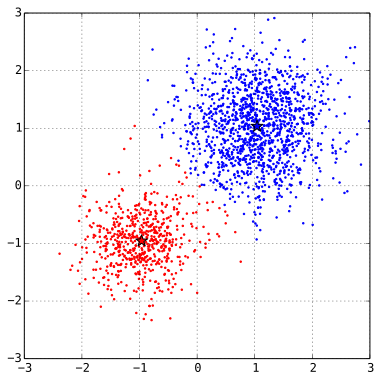
\includegraphics[width=.5\linewidth]{images/gmm.km.k2.eps}}
\subfloat[$K=3$.]{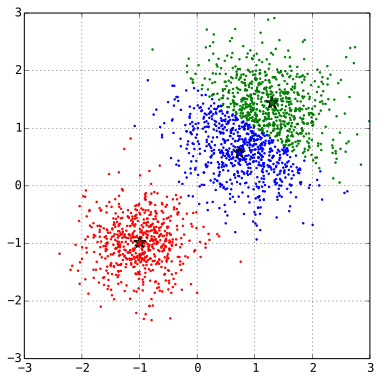
\includegraphics[width=.5\linewidth]{images/gmm.km.k3.eps}}
\caption{$k$-means clustering on Gaussian mixture model.\label{fig:kmean}}
\end{figure}

なお、正規分布の分散を考慮せず、同じ広がりを持つ集団を想定した点が、課題である。その様子は\figref{kmean}にも窺える。

\section{期待値最大化法の理論\label{sect:em}}

\sectref{em}では、潜在変数$z$を、その値が確率的に決まる\textbf{確率変数}と考え、分散を含む、混合正規分布の母数を推定しよう。
観測変数$\bm{x}$に対し、潜在変数$z$の確率は、\eqref{em:estep}で求まる。観測に基づき推定した確率なので、これを事後確率と呼ぶ。
%
\begin{equation}
\label{eq:em:estep}
\Prob{z_{nk}}[\bm{x}_n,\theta] = \frac{w_k \Nd{\bm{x}_n}{\bm{\mu}_k,S_k}}{\prob{\bm{x}_n}} = \gamma_{nk}.
\end{equation}
%
次に、混合正規分布の尤度を定義する。尤度$\Lk{\theta}$は母数$\theta$の妥当性を表し、尤度の最大値を探す操作が最尤推定である。
%
\begin{equation}
\label{eq:em:L}
\Lk{\theta} =
\Prob{\bm{x}}[\theta] =
\prod_{n=1}^N \sum_{k=1}^K w_k \Nd{\bm{x}_n}{\bm{\mu}_k,S_k}.
\end{equation}
%
微分計算の都合により、尤度を対数化して、対数尤度を最小化する母数を計算しよう。重心$\bm{\mu}_k$による偏微分の例を示す。
%
\begin{equation}
\label{eq:em:L:m}
\pdiff{}{\bm{\mu}_k}\log\Lk{\theta} =
\pdiff{}{\bm{\mu}_k}\sum_{n=1}^N \log\sum_{k=1}^K w_k \Nd{\bm{x}_n}{\bm{\mu}_k,S_k} =
\sum_{n=1}^N \gamma_{nk} S_k^{-1} (\bm{x}_n - \bm{\mu}_k).
\end{equation}
%
加重と重心と分散の推定値$\hat{w}_k,\hat{\bm{\mu}}_k,\hat{S}_k$は\eqref{em:mstep}となる。加重のみ、\eqref{gmm}より、\textbf{ラグランジュの未定乗数法}で求めた。
%
\begin{equation}
\label{eq:em:mstep}
\hat{w_k} = \frac{N_k}{N},\esp
\left\{
\begin{aligned}
\hat{\bm{\mu}_k} &= \frac{1}{N_k} \sum_{n=1}^N \gamma_{nk} \bm{x}_n,\\
\hat{S_k} &= \frac{1}{N_k} \sum_{n=1}^N \gamma_{nk} (\bm{x}_n - \hat{\bm{\mu}}_k) \trans{(\bm{x}_n - \hat{\bm{\mu}}_k)},
\end{aligned}
\right\}
\where
N_k = \sum_{n=1}^N \gamma_{nk}.
\end{equation}
%
\eqref{em:mstep}より、事後確率$\gamma$が求まれば、母数も求まるが、\eqref{em:estep}より、事後確率$\gamma$の計算には、母数の値が必要である。
従って、解析的な求解は困難である。ここで、凸関数$f$と、正の実数$\gamma_n$は、\eqref{jensen}の\textbf{イェンゼンの不等式}を満たす。
%
\begin{equation}
\label{eq:jensen}
\sum_{n=1}^N \gamma_n f(x_n) \geq f\tup{\sum_{n=1}^N \gamma_n x_n},
\where
\sum_{n=1}^N \gamma_n=1.
\end{equation}
%
対数が凹関数である点に注意して、\eqref{jensen}に\eqref{em:L}を代入して、\eqref{em:jensen}の関数$Q$を得る。これを\textbf{補助関数}と呼ぶ。
%
\begin{equation}
\label{eq:em:jensen}
\log \Lk{\theta} =
\max_\gamma Q(\gamma,\theta) \geq
\sum_{n=1}^N \sum_{k=1}^K \gamma_{nk} \log \frac{w_k \Nd{\bm{x}_n}{\bm{\mu}_k,S_k}}{\gamma_{nk}} =
Q(\gamma,\theta).
\end{equation}
%
補助関数$Q$は、\eqref{em:Q}に示す、変数$\gamma,\theta$の修正を交互に繰り返すと単調増加し、最終的に、有限な実数値に収束する。
%
\begin{equation}
\label{eq:em:Q}
\left\{
\begin{aligned}
\hat{\gamma}^{t+1} &= \argmax_{\gamma} Q(\gamma,\theta^t), \\
\hat{\theta}^{t+1} &= \argmax_{\theta} Q(\gamma^t,\theta).
\end{aligned}
\right.
\end{equation}
%
\eqref{em:Q}で、変数$\gamma^t,\theta^t$の最適値を求めると、\eqref{em:estep}と\eqref{em:mstep}を得る。両者を交互に修正すると、尤度が最大化する。
\eqref{em:estep}で変数$\gamma$を修正する操作は、\eqref{em:L:exp}に示す、対数尤度の期待値を計算する操作である。これを\Estep{}と呼ぶ。
%
\begin{equation}
\label{eq:em:L:exp}
\E[z]{\log \Prob{\bm{x},z}[\theta]} =
\int_z \Prob{z}[\bm{x},\theta] \log \Prob{\bm{x},z}[\theta] dz =
\sum_{n=1}^N \sum_{k=1}^K \gamma_{nk} \log \seq{w_k \Nd{\bm{x}_n}{\bm{\mu}_k,S_k}}.
\end{equation}
%
\eqref{em:mstep}で変数$\theta$を修正する操作は、尤度を最大化する。これを\Mstep{}と呼び、両者を合わせて\textbf{期待値最大化法}と呼ぶ。
なお、単位行列$E$と実数値$\lambda$を使って、分散を$\lambda E$と置くと、極限$\lambda\to0$で\eqref{km:elog}が成立し、変数$\gamma_{nk}$も$z_{nk}$になる。
%
\begin{equation}
\label{eq:km:elog}
\lim_{\lambda\to0} \lambda\log \seq{w \Nd{\bm{x}}{\bm{\mu},\lambda E}} =
\lim_{\lambda\to0} \seq{\lambda\log w - \lambda\frac{D}{2} \log (2\pi\lambda) - \frac{1}{2} \norm{\bm{x}-\bm{\mu}}^2} =
-\frac{1}{2} \norm{\bm{x}-\bm{\mu}}^2.
\end{equation}
%
即ち、\eqref{km:L}が成立し、その最大化は\eqref{km:D}の最小化に帰結する。\kmean{}は、期待値最大化法の特殊な例と言える。
%
\begin{equation}
\label{eq:km:L}
\lim_{\lambda\to0} \lambda \E[\bm{z}]{\log \Prob{\bm{x},z}[\theta]} =
-\frac{1}{2} \sum_{n=1}^N \sum_{k=1}^K z_{nk} \norm{\bm{x}_n-\bm{\mu}_k}^2.
\end{equation}
%
また、期待値最大化法も、\sectref{vb}で学ぶ変分ベイズ法の特殊な場合であり、\sectref{em}と酷似した式が、何度か登場する。

\section{期待値最大化法の実装}

\sectref{em}の議論に基づき、期待値最大化法を実装する。まず、$K$個の$D$変量正規分布からなる混合正規分布を実装する。

\begin{Verbatim}{Scala}
class GMM(val d: Int, val k: Int) {
	val w = Array.fill(k)(1.0 / k)
	val m -> s = (Array.fill(k, d)(math.random), Array.fill(k, d)(math.random))
	def apply(x: Seq[Double]) = w.lazyZip(m).lazyZip(s).map(Normal(x)(_,_,_).p)
}
\end{Verbatim}

正規分布も実装する。引数は、加重と平均と分散である。なお、分散共分散行列を対角行列と仮定し、実装を単純化した。

\begin{Verbatim}{Scala}
case class Normal(x: Seq[Double])(w: Double, m: Seq[Double], s: Seq[Double]) {
	def n = math.exp(-0.5 * x.zip(m).map(_-_).map(d=>d*d).zip(s).map(_/_).sum)
	def p = w * n / math.pow(2 * math.Pi, 0.5 * x.size) / math.sqrt(s.product)
}
\end{Verbatim}

次に、最適化の手順を実装する。期待値最大化法の\Estep{}と\Mstep{}を繰り返す。また、点$\bm{x}$が属す集団$C_k$を推定する。

\begin{Verbatim}{Scala}
class EM(val x: Seq[Seq[Double]], val mm: GMM, epochs: Int = 100) {
	def mstep(P: Seq[Seq[Double]]) = {
		P.map(_.sum / x.size).copyToArray(mm.w)
		val m = P.map(_.zip(x).map((p,x) => x.map(x => p * x)).transpose.map(_.sum))
		val s = P.map(_.zip(x).map((p,x) => x.map(x => p*x*x)).transpose.map(_.sum))
		m.zip(P).map((m,p) => m.map(_ / p.sum)).zip(mm.m).foreach(_.copyToArray(_))
		s.zip(P).map((s,p) => s.map(_ / p.sum)).zip(mm.s).foreach(_.copyToArray(_))
		for((s,m) <- mm.s.zip(mm.m); d <- 0 until mm.d) s(d) -= m(d) * m(d)
	}
	for(epoch <- 1 to epochs) mstep(x.map(mm(_)).map(p=>p.map(_/p.sum)).transpose)
}
\end{Verbatim}

\figref{em}は、\figref{gmm}と同じ散布図を、期待値最大化法で学習した結果で、\figref{gmm}と同様に、確率密度関数を可視化した。

\begin{figure}[h]
\centering
\subfloat[$K=2$.]{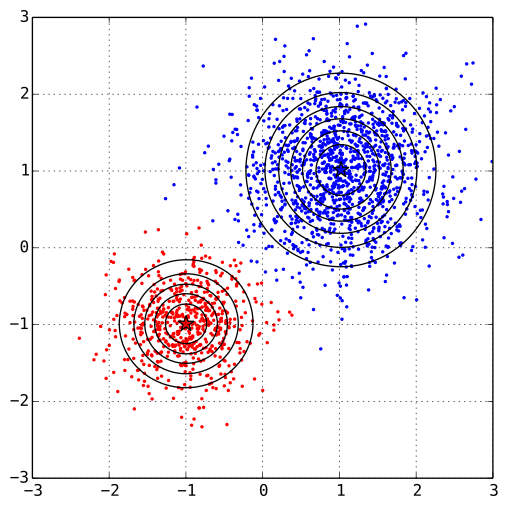
\includegraphics[width=.5\linewidth]{images/gmm.em.k2.eps}}
\subfloat[$K=3$.]{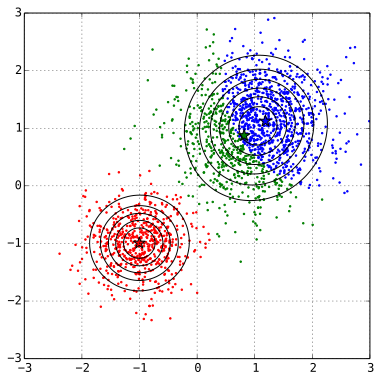
\includegraphics[width=.5\linewidth]{images/gmm.em.k3.eps}}
\caption{expectation maximization on a Gaussian mixture model.\label{fig:em}}
\end{figure}

期待値最大化法では、\figref{kmean}の\kmean{}と比較して、正規分布の密度の強弱を、境界付近の色分けに正しく反映できる。

\section{変分ベイズ推定の理論\label{sect:vb}}

\sectref{em}の最尤推定では、母数の最適値を推定した。\sectref{vb}で議論するベイズ推定では、母数の確率分布を推定できる。
特に、最適解が複数ある場合にも対応でき、過学習の抑制効果も期待できる。議論を始めるに当たり、尤度を定義しよう。
%
\begin{equation}
\label{eq:vb:L}
\Lk{\theta} =
\prob{\bm{x}}[\theta] =
\int \prob{\bm{x},z} dz =
\int \prob{\bm{x}}[z] \prob{z}[\theta] dz.
\end{equation}
%
\sectref{vb}では、潜在変数$z$に加え、母数$\theta$も確率変数に含める。母数$\theta$の確率分布に母数$\phi$を設定し、尤度を定義し直す。
%
\begin{equation}
\label{eq:vb:Lm}
\Lk{\phi} =
\prob{\bm{x}}[\phi] =
\iint \prob{\bm{x},z,\theta}[\phi] dz d\theta =
\iint \prob{\bm{x}}[z] \prob{z}[\theta] \prob{\theta}[\phi] dz d\theta.
\end{equation}
%
\eqref{vb:L}に対し、\eqref{vb:Lm}を\textbf{周辺尤度}と呼ぶ。\sectref{em}と同様に、補助関数$F$を定義する。関数$\hatp$は、適当な分布である。
%
\begin{equation}
\log \Lk{\phi} =
\log \iint \hatprob{z,\theta} \frac{\prob{\bm{x},z,\theta}}{\hatprob{z,\theta}} dz d\theta \geq
\iint \hatprob{z,\theta} \log \frac{\prob{\bm{x},z,\theta}}{\hatprob{z,\theta}} dz d\theta = F(\hatp).
\end{equation}
%
補助関数$F$を最大化すると、尤度$\Lp$に収束する。その差は、\eqref{vb:KL}に示す\textbf{カルバック・ライブラー情報量}の形になる。
\eqref{vb:KL}は、変数$z,\theta$が従う分布$\hatp$を仮定した場合の、分布$\hatp,p$の平均情報量の差である。両者が同じ場合に$0$となる。
%
\begin{equation}
\label{eq:vb:KL}
\log \Lk{\bm{x}} - F(\hatp) =
\iint \hatprob{z,\theta} \log \prob{\bm{x}} dz d\theta - F(\hatp) =
\iint \hatprob{z,\theta} \log \frac{\hatprob{z,\theta}}{\prob{z,\theta}[\bm{x}]} dz d\theta =
\KL{\hatp}{p} \geq 0.
\end{equation}
%
関数$\hatp$を引数に取る関数$F$を、\textbf{汎関数}と呼ぶ。汎関数$F$の極値を与える引数$\hatp$を探索する問題は、\textbf{変分問題}と呼ばれる。
残念ながら、複数の引数を取る関数$\hatp$の探索は難しく、\eqref{vb:field}に示す\textbf{平均場近似}により、変数間の独立性を仮定する。
%
\begin{equation}
\label{eq:vb:field}
\hatprob{z,\theta} = f(z)g(\theta),
\where
\left\{
\begin{aligned}
\int f(z) dz &= 1,\\
\int g(\theta) d\theta &= 1.
\end{aligned}
\right.
\end{equation}
%
関数$f,g$に対する汎関数$F$の変分問題を解く。ここで、\eqref{vb:EL}に示す\textbf{オイラー・ラグランジュ方程式}の特殊形を使う。
%
\begin{equation}
\label{eq:vb:EL}
\pdiff{}{f} \pdiff{F}{z} =
\pdiff{}{f} \int f(z) g(\theta) \log \frac{\prob{\bm{x},z,\theta}}{f(z)g(\theta)} d\theta = 0.
\end{equation}
%
関数$f$の値を固定し、単に変数と考えて偏微分すると、\eqref{vb:EL:sol}を得る。関数$g$に対し、\eqref{vb:field}の制約条件を使った。
%
\begin{equation}
\label{eq:vb:EL:sol}
\pdiff{}{f} \int f(z) g(\theta) \log \frac{\prob{\bm{x},z,\theta}}{f(z)g(\theta)} d\theta =
\int g(\theta) \log \frac{\prob{\bm{x},z,\theta}}{f(z)g(\theta)} d\theta - 1 = 0.
\end{equation}
%
\eqref{vb:EL:sol}から、関数$f$の最適値を求める。\eqref{vb:field}の近似で仮定した、変数$z,\theta$間の独立性より、\eqref{vb:logf}が成立する。
%
\begin{equation}
\label{eq:vb:logf}
\log f(z) =
\log f(z) \int g(\theta) d\theta =
\int g(\theta) \log f(z) d\theta.
\end{equation}
%
関数$f,g$の最適値$\hat{f},\hat{g}$は、\eqref{vb:em}となる。関数$f,g$を交互に修正すると、補助関数$F$が増加し、周辺尤度に収束する。
\eqref{vb:em}は、\eqref{em:Q}の\Estep{}と\Mstep{}に対応し、\sectref{em}で学んだ期待値最大化法に対し、\textbf{変分ベイズ法}と呼ばれる。
%
\begin{equation}
\label{eq:vb:em}
\left\{
\begin{alignedat}{2}
\hat{f}(z) &\propto \exp \int g(\theta) \log \prob{\bm{x},z,\theta} d\theta &&= \exp \E[g]{\log \prob{\bm{x},z,\theta}},\\
\hat{g}(\theta) &\propto \exp \int f(z) \log \prob{\bm{x},z,\theta} dz &&= \exp \E[f]{\log \prob{\bm{x},z,\theta}}.
\end{alignedat}
\right.
\end{equation}
%
なお、母数$\theta$に対し、適当な事前分布を設定すると、分布$\hat{g}$と事前分布$p$の乖離を抑制し、過学習を防ぐ効果が生じる。
%
\begin{equation}
\label{eq:vb:penalty}
F(\hatp) =
\iint f(z)g(\theta) \log \frac{\prob{\bm{x},z}[\theta]}{f(z)} \frac{\prob{\theta}}{g(\theta)} dz d\theta =
\E[f,g]{\log \frac{\prob{\bm{x},z}[\theta]}{f(z)}} - \KL{g(\theta)}{\prob{\theta}}.
\end{equation}
%
無限の個数の点$\bm{x}_n$を学習した場合の尤度は、\textbf{ラプラス近似}で\eqref{vb:BIC}と近似でき、\textbf{ベイズ情報量基準}の形が出現する。
%
\begin{equation}
\label{eq:vb:BIC}
F(\hatp) \simeq
\E[f,g]{\log \frac{\prob{\bm{x},z}[\theta]}{f(z)}} - \frac{\hat{\abs{\theta}}}{2} \log N + \log \prob{\hat{\theta}}.
\end{equation}
%
\eqref{vb:BIC}には、疎な基底を学習し、母数の個数$\abs{\theta}$を実質的に削減する\textbf{正則化}の効果があり、過学習の抑制が期待できる。

\section{母数の事前分布の設定\label{sect:vbgmm}}

潜在変数$z$や母数$\theta$の事前分布を注意深く設定すると、事前分布と事後分布が同じ形の分布になり、計算が容易になる。
これを\textbf{共役分布}と呼ぶ。混合正規分布の母数にも、共役分布が存在する。まず、潜在変数$z$が多項分布に従うと仮定する。
%
\begin{equation}
\label{eq:vbgmm:p:z}
\prob{z}[w] = \prod_{n=1}^N \prod_{k=1}^K w_k^{z_{nk}},
\where
\forall n\colon
\sum_{k=1}^K z_{nk} = 1.
\end{equation}
%
\eqref{vbgmm:p:z}は、潜在変数$z$に対する加重$w$の尤度でもある。加重$w$の事前分布を、\eqref{vbgmm:p:w}のディリクレ分布で定義する。
これは、$K$個の排反事象の反復試行で、事象$k$の出現が$\alpha_k-1$回だった場合に、事象$k$の確率が$w_k$である確率を表す。
%
\begin{equation}
\label{eq:vbgmm:p:w}
\prob{w} = \Dd{w}{\alpha} =
\Gd{\sum_{k=1}^K \alpha_k} \prod_{k=1}^K \frac{w_k^{\alpha_k-1}}{\Gd{\alpha_k}} =
\frac{1}{\Bd{\alpha}} \prod_{k=1}^K w_k^{\alpha_k-1}.
\end{equation}
%
関数$\Gp$はガンマ関数で、階乗を拡張した複素関数である。関数$\Bp$はベータ関数で、多項係数を拡張した複素関数である。
平均$\bm{\mu}$の事前分布には、\eqref{vbgmm:p:m}の正規分布を仮定する。母数$\sigma$には、\eqref{vbgmm:p:m}の分散を徐々に減少させる効果がある。
%
\begin{equation}
\label{eq:vbgmm:p:m}
\prob{\bm{\mu}}[S] = \prod_{k=1}^K \Nd{\bm{\mu}_k}{\bm{m}_k,\sigma_k^{-1} S_k}.
\end{equation}
%
\eqref{vbgmm:p:m}は、平均$\bm{\mu}$に対する分散$S$の尤度でもある。分散$S$の事前分布は、\eqref{vbgmm:p:S}の\textbf{逆ウィシャート分布}を仮定する。
%
\begin{equation}
\label{eq:vbgmm:p:S}
\prob{S} =
\prod_{k=1}^K \Wd{S_k^{-1}}{W_k,\nu_k} =
\prod_{k=1}^K \frac{1}{\Wn{W_k,\nu_k}} \abs{S_k^{-1}}^{\FRAC{\nu_k-D-1}{2}} \exp\seq{-\frac{1}{2}\trace{W_k^{-1}S_k^{-1}}}.
\end{equation}
%
これは、分散$W$の$D$変量正規分布に従う$\nu$個の変数$\bm{x}_n$の直積$\bm{x}_n\trans{\bm{x}_n}$の和の分布である。即ち、標本分散の分布である。
%
\begin{equation}
\Wn{W_k,\nu_k} = 2^{\FRAC{\nu_kD}{2}} \pi^{\FRAC{D(D-1)}{4}} \abs{W_k}^{\FRAC{\nu_k}{2}} \prod_{d=0}^{D-1} \Gd{\frac{\nu_k-d}{2}}.
\end{equation}
%
\figref{vb}は、\figref{gmm}と同じ散布図を、変分ベイズ法で学習した結果で、\figref{gmm}と同様に、確率密度関数を可視化した。

\begin{figure}[h]
\centering
\subfloat[$K=2$.]{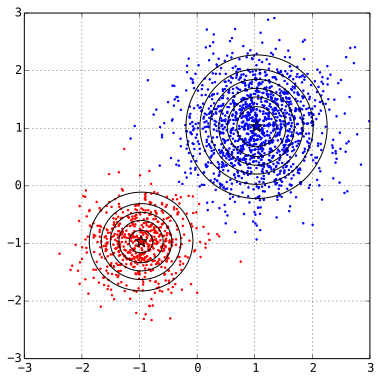
\includegraphics[width=.5\linewidth]{images/gmm.vb.k2.eps}}
\subfloat[$K=3$.]{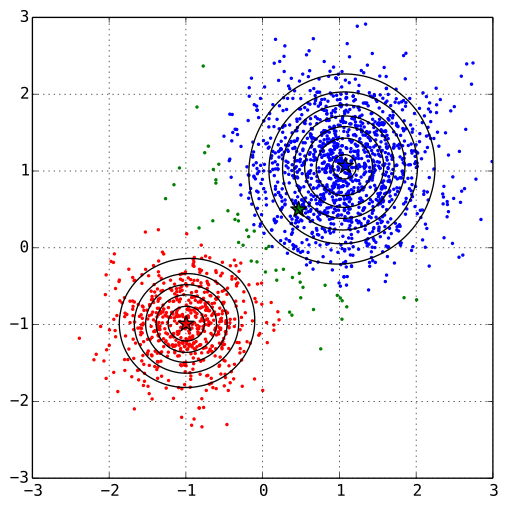
\includegraphics[width=.5\linewidth]{images/gmm.vb.k3.eps}}
\caption{variational Bayesian inference on a Gaussian mixture model.\label{fig:vb}}
\end{figure}

正則化の恩恵により、集団の個数を過剰に設定した場合でも、余剰の集団の加重が徐々に低下し、過学習が抑制される。

\section{母数の事後分布の導出}

変分ベイズ法の\eqref{vb:em}に対し、\sectref{vbgmm}で設定した共役事前分布を代入する。まず、全ての変数の結合確率を求める。
%
\begin{equation}
\prob{\bm{x},z,w,\bm{\mu},S} =
\prob{\bm{x},z}[w,\bm{\mu},S] \prob{w,\bm{\mu},S} =
\prob{\bm{x}}[z,\bm{\mu},S] \prob{z}[w] \prob{w) \prob{\bm{\mu}}[S] p(S}.
\end{equation}
%
\Estep{}を導く。母数$\theta$の事前分布を固定し、潜在変数$z$の分布を最適化する操作なので、その間に\eqref{vbgmm:estep}が成立する。
%
\begin{equation}
\label{eq:vbgmm:estep}
f(z) \propto
\exp \E[g]{\log \prob{\bm{x},z}[w,\bm{\mu},S]} =
\exp \sum_{n=1}^N \sum_{k=1}^K z_{nk} \seq{\E[w]{\log w_k} + \E[\bm{\mu},S]{\log \Nd{\bm{x}_n}{\bm{\mu}_k,S_k}}} \propto
\prod_{n=1}^N \prod_{k=1}^K \gamma_{nk}^{z_{nk}}.
\end{equation}
%
\eqref{vbgmm:estep}に現れる、加重$w$の対数の期待値は、\eqref{vbgmm:estep:w}となる。関数$\Pp$は\textbf{ディガンマ関数}で、関数$\Gp$の対数微分である。
%
\begin{equation}
\label{eq:vbgmm:estep:w}
\E[w]{\log w_k} =
\frac{1}{\Bd{\alpha}} \pdiff{}{\alpha_k} \int \prod_{j=1}^K w_j^{\alpha_j-1} dw =
\pdiff{}{\alpha_k} \log \Bd{\alpha} =
\Pd{\alpha_k} - \Pd{\sum_{j=1}^K \alpha_j}.
\end{equation}
%
\eqref{vbgmm:estep}に現れる、正規分布の対数の期待値は、\eqref{gmm:n}の正規分布の確率密度関数より、\eqref{vbgmm:estep:n}の形に分解できる。
%
\begin{equation}
\label{eq:vbgmm:estep:n}
\E[\bm{\mu},S]{\log \Nd{\bm{x}_n}{\bm{\mu}_k,S_k}} =
- \frac{1}{2} \E[\bm{\mu},S]{D \log 2\pi + \log \abs{S_k} + \trans{(\bm{x}_n - \bm{\mu}_k)} S_k^{-1} (\bm{x}_n - \bm{\mu}_k)}.
\end{equation}
%
\eqref{vbgmm:estep:n}に現れる、行列式$\abs{S}$の対数の期待値は、\eqref{vbgmm:p:S}の確率密度関数を母数$\nu_k$で偏微分すれば、\eqref{vbgmm:estep:det}となる。
%
\begin{equation}
\label{eq:vbgmm:estep:det}
\E[S]{\log \abs{S_k}} =
2 \int \pdiff{\Wt}{\nu_k}\frac{\Wp}{\Wt} dS - 2 \int \pdiff{\Wp}{\nu_k} dS =
\frac{2}{\Wt} \pdiff{\Wt}{\nu_k} =
- D\log 2 - \log\abs{W_k} - \sum_{d=0}^{D-1} \Pd{\frac{\nu_k-d}{2}}.
\end{equation}
%
\eqref{vbgmm:estep:n}に現れる、行列積の期待値は、母数$\bm{\mu}$が、\eqref{vbgmm:p:m}の正規分布に従う事実と因数分解により、\eqref{vbgmm:estep:S}となる。
%
\begin{equation}
\label{eq:vbgmm:estep:S}
\E[\bm{\mu},S]{\trans{(\bm{x}_n - \bm{\mu}_k)} S_k^{-1} (\bm{x}_n - \bm{\mu}_k)} =
\nu_k \trans{(\bm{x}_n - \bm{m}_k)} W_k (\bm{x}_n - \bm{m}_k) + \frac{D}{\sigma_k}.
\end{equation}
%
\Mstep{}を導く。事後確率$\gamma$を\eqref{vbgmm:mstep}に代入し、事前分布と事後分布の共役性に注意して、母数の事後分布を求めよう。
%
\begin{equation}
\label{eq:vbgmm:mstep}
g(\theta) \propto \exp\seq{\E[z]{\log \prob{\bm{x},z}[w,\bm{\mu},S]} + \log \prob{w) + \log \prob{\bm{\mu}}[S] + \log p(S}}.
\end{equation}
%
\eqref{vbgmm:mstep}で、変数$\bm{x},z$の結合確率の対数の期待値は、\eqref{gmm:n}の正規分布と\eqref{vbgmm:p:z}の多項分布より、\eqref{vbgmm:mstep:xz}となる。
%
\begin{equation}
\label{eq:vbgmm:mstep:xz}
\E[z]{\log \prob{\bm{x},z}[w,\bm{\mu},S]} =
- \frac{1}{2} \sum_{k=1}^K \sum_{n=1}^N \gamma_{nk}
\seq{D \log 2\pi + \abs{S_k} + \trans{(\bm{x}_n-\hat{\bm{\mu}}_k)} S_k^{-1} (\bm{x}_n-\hat{\bm{\mu}}_k) - 2 \log w_k}.
\end{equation}
%
共役性より、母数$\theta$の事後分布は、事前分布の母数$\phi$を、推定値$\hat{\phi}$に置換した場合と等値であり、\eqref{vbgmm:mstep:wmS}が成立する。
%
\begin{equation}
\label{eq:vbgmm:mstep:wmS}
\E[z]{\log \prob{\theta}[\bm{x},z]} =
\log \prob{\theta}[\hat{\phi}] =
\E[z]{\log \prob{\bm{x},z}[\theta]} + \log \prob{\theta}[\phi] - \E[z]{\log \prob{\bm{x},z}}.
\end{equation}
%
\eqref{vbgmm:mstep:wmS}より、母数$\alpha,\sigma,\nu$の推定値に対して、\eqref{vbgmm:mstep:N}が成立する。変数$N_k$は、集団$C_k$の要素の個数の期待値を表す。
%
\begin{equation}
\label{eq:vbgmm:mstep:N}
\hat{\alpha}_k - \alpha_k = \hat{\sigma}_k - \sigma_k = \hat{\nu}_k - \nu_k = N_k = \sum_{n=1}^N z_{nk}.
\end{equation}
%
母数$\bm{m}$の場合は、\eqref{vbgmm:mstep:m}が成立する。期待値最大化法の\eqref{em:mstep}を考えれば、事前分布と標本平均の加重平均である。
%
\begin{equation}
\label{eq:vbgmm:mstep:m}
\hat{\bm{m}}_k = \frac{1}{\hat{\sigma}_k} \tup{\sigma_k \bm{m}_k + \sum_{n=1}^N \gamma_{nk} \bm{x}_n}.
\end{equation}
%
母数$W$の場合は、\eqref{vbgmm:mstep:W}が成立する。これも、\eqref{vbgmm:mstep:W}の右辺に着目すれば、事前分布と標本分散の加重平均である。
%
\begin{equation}
\label{eq:vbgmm:mstep:W}
\hat{W}_k^{-1} =
W_k^{-1}+\sum_{n=1}^N\gamma_{nk}\bm{x}_n\trans{\bm{x}_n}+\sigma_k\bm{m}_k\trans{\bm{m}_k}-\hat{\sigma}_k\hat{\bm{m}}_k\trans{\hat{\bm{m}}_k}.
\end{equation}
%
\eqref{vbgmm:mstep:W}の導出では、分散$W$の\textbf{コレスキー分解}により下三角行列$T$が存在して、\eqref{vbgmm:trace}が成立する性質を利用した。
%
\begin{equation}
\label{eq:vbgmm:trace}
\trans{\bm{x}} W \bm{x} =
(\trans{\bm{x}} T) (\trans{T} \bm{x}) =
\trans{(\trans{T} \bm{x})} (\trans{T} \bm{x}) =
\trace{(\trans{T} \bm{x}) \trans{(\trans{T} \bm{x})}} =
\trace{\trans{T} (\bm{x} \trans{\bm{x}}) T} =
\trace{(\bm{x} \trans{\bm{x}}) W}.
\end{equation}
%
事前分布と最尤推定の最適値の加重平均が現れる点には、\eqref{vb:penalty}で議論した、事前分布による正則化の効果が窺える。

\section{変分ベイズ推定の実装}

\sectref{vbgmm}の議論に基づき、変分ベイズ推定を実装する。まず、本体を実装する。引数は、期待値最大化法と同等である。
\eqref{vbgmm:mstep:N}より、母数$\alpha,\sigma,\nu$は、初期値を揃えると、以後の最適化を通じて常に同じ値になる。そこで、同じ変数にした。

\begin{Verbatim}{Scala}
class VB(val x: Seq[Seq[Double]], val mm: GMM, epochs: Int = 1000, W: Double = 1) {
	val n = Array.fill(mm.k)(1.0 / mm.k)
	val w -> m = (Array.fill(mm.k, mm.d)(W), Array.fill(mm.k, mm.d)(math.random))
	for(epoch <- 1 to epochs) new MstepGMM(this, mm, new EstepGMM(this, mm).post)
}
\end{Verbatim}

\Estep{}を実装する。\eqref{vbgmm:estep}に基づき、潜在変数$z$の事後確率$\gamma$を計算する。最後に、総和で事後確率$\gamma$を規格化する。

\begin{Verbatim}{Scala}
class EstepGMM(vb: VB, mm: GMM) {
	val eq35 = vb.n.map(Digamma).map(_-Digamma(vb.n.sum))
	val eq3A = vb.n.map(n=>0.to(mm.d-1).map(d=>(n-d)/2).map(Digamma))
	val eq36 = eq3A.zip(vb.w).map(_.sum-_.map(math.log).sum).map(_/2)
	def wish = vb.x.toArray.map(_.toArray).map(vb.m-_).map(d=>d.mul(d).div(vb.w))
	def eq34 = wish.map(_.zip(vb.n).map(-_.sum/2*_))+eq35+eq36-vb.n.map(mm.d/_/2)
	def post = eq34.map(_.map(math.exp)).map(x=>x.map(_/x.sum)).toSeq.transpose
}
\end{Verbatim}

\Mstep{}を実装する。期待値最大化法の実装を流用して、母数の最尤推定値を計算し、事前分布との加重平均を計算する。

\begin{Verbatim}{Scala}
class MstepGMM(vb: VB, mm: GMM, post: Seq[Seq[Double]]) {
	new EM(vb.x, mm, 0).mstep(post)
	val eq11 = post.map(_.sum).toArray
	val eq38 = vb.n.zip(eq11).map(_+_)
	val eq39 = vb.m.mul(vb.n).div(eq38).add(mm.m.mul(eq11).div(eq38))
	val eq41 = vb.m.mul(vb.m).mul(vb.n).sub(eq39.mul(eq39).mul(eq38))
	val eq40 = mm.s.add(mm.m.mul(mm.m)).mul(eq11).add(vb.w.add(eq41))
	eq38.copyToArray(vb.n)
	eq39.zip(vb.m).foreach(_.copyToArray(_))
	eq40.zip(vb.w).foreach(_.copyToArray(_))
}
\end{Verbatim}

\Mstep{}では、平均や分散の配列の四則演算が頻繁に現れる。簡潔な実装を目指し、暗黙の型変換で四則演算を実現した。

\begin{Verbatim}{Scala}
implicit class Vector(x: Array[Array[Double]]) {
	def +(y: Array[Double]) = x.map(_.zip(y).map(_+_))
	def -(y: Array[Double]) = x.map(_.zip(y).map(_-_))
	def add(y: Array[Double]) = x.zip(y).map((x,y) => x.map(_+y))
	def sub(y: Array[Double]) = x.zip(y).map((x,y) => x.map(_-y))
	def mul(y: Array[Double]) = x.zip(y).map((x,y) => x.map(_*y))
	def div(y: Array[Double]) = x.zip(y).map((x,y) => x.map(_/y))
	def add(y: Array[Array[Double]]) = x.zip(y).map(_.zip(_).map(_+_))
	def sub(y: Array[Array[Double]]) = x.zip(y).map(_.zip(_).map(_-_))
	def mul(y: Array[Array[Double]]) = x.zip(y).map(_.zip(_).map(_*_))
	def div(y: Array[Array[Double]]) = x.zip(y).map(_.zip(_).map(_/_))
}
\end{Verbatim}

最後に、ディガンマ関数を実装する。詳細は省くが、\textbf{ワイエルシュトラスの無限乗積表示}を利用して、簡単に計算できる。

\begin{Verbatim}{Scala}
object Digamma extends Function[Double, Double] {
	def apply(x: Double): Double = {
		var index -> value = (x, 0.0)
		def d = 1.0 / (index * index)
		while(index < 49) (value -= 1 / index, index += 1)
		val s = d * (1.0 / 12 - d * (1.0 / 120 - d / 252))
		(value + math.log(index) - 0.5 / index - s)
	}
}
\end{Verbatim}

\end{document}
